% Opcje klasy 'iithesis' opisane sa w komentarzach w pliku klasy. Za ich pomoca
% ustawia sie przede wszystkim jezyk oraz rodzaj (lic/inz/mgr) pracy.
\documentclass[shortabstract, english, inz]{iithesis}

\usepackage[utf8]{inputenc}
\usepackage{minted}

%%%%% DANE DO STRONY TYTUŁOWEJ
% Niezaleznie od jezyka pracy wybranego w opcjach klasy, tytul i streszczenie
% pracy nalezy podac zarowno w jezyku polskim, jak i angielskim.
% Pamietaj o madrym (zgodnym z logicznym rozbiorem zdania oraz estetyka) recznym
% zlamaniu wierszy w temacie pracy, zwlaszcza tego w jezyku pracy. Uzyj do tego
% polecenia \fmlinebreak.
\polishtitle    {Porównanie wydajności \fmlinebreak różnych implementacji algorytmu Wave Function Collapse}
\englishtitle   {Performance comparison of Wave Function Collapse Algorithm implementations}
\polishabstract {Algorytm Wave Function Collapse (WFC) autorstwa Maxim'a Gumin'a służy do proceduralnego tworzenia treści (ang. procedural content generation PCG) w oparciu o przykładowe obrazy i jest przykładem algorytmu probabilistycznego. Dla uzyskania podobieństwa pomiędzy danymi wejściowymi a wynikiem, algorytm syntezuje obraz z fragmentów wejścia przestrzegając zasad sąsiedztwa z oryginalnego obrazu. Ta praca opisuje zasady działania WFC, jego zastosowania i analizę wydajności różnych implementacji wariantu algorytmu służącego do tworzenia trójwymiarowego modelu w oparciu o predefiniowany zestaw klocków (ang. tileset). Dodatkowo zawiera autorskie pomysły na poprawę wydajności tego algorytmu. Wszystkie wymienione wersje algorytmu zostały zaimplementowane i przetestowane w ramach tej pracy. Podczas testów okazało się, że nasze rozwiązanie ma znacząco mniejszy czas wykonania, a złożoność obliczeniowa algorytmu została zmniejszona o rząd wielkości. \fmlinebreak \fmlinebreak
Repozytorium projektu:\fmlinebreak
\url{https://github.com/KrzysiekSlawik/wfc}}
\englishabstract{The Wave Function Collapse (WFC) algorithm, created by Maxim Gumin, can be used for procedural content generation (PCG), and it is an example of a probabilistic algorithm. Its input is an example image, and its output is an image that follows the input style by using parts of the example image and respecting the neighbor relations between them. This paper aims to describe the theory behind the WFC, where it can be applied, and to compare the performance of different implementations of the WFC variants that serve as tilemap generators.
Additionally, it includes our original ideas for improving the algorithm's performance. All mentioned variants were implemented in Rust and benchmarked under the same conditions. During the tests, it turned out that our original approach improved performance  and the time complexity got reduced.}
% w pracach wielu autorow nazwiska mozna oddzielic poleceniem \and
\author         {Krzysztof Sławik}
% w przypadku kilku promotorow, lub koniecznosci podania ich afiliacji, linie
% w ponizszym poleceniu mozna zlamac poleceniem \fmlinebreak
\advisor        {dr Łukasz Piwowar}
\date          {03.02.2023}                     % Data zlozenia pracy
% Dane do oswiadczenia o autorskim wykonaniu
\transcriptnum {307020}                     % Numer indeksu
\advisorgen    {dr. Łukasza Piwowara} % Nazwisko promotora w dopelniaczu
%%%%%

%%%%% WLASNE DODATKOWE PAKIETY
%
\usepackage{amsmath,amssymb,amsthm,amsfonts}

\usepackage{booktabs}
\usepackage{enumitem}
\setlist{nosep}
\usepackage{url}
\usepackage{graphicx}
\usepackage{float}
\usepackage{subcaption}
\usepackage[language=english]{biblatex}
\addbibresource{bibliography.bib}

%%%%% WŁASNE DEFINICJE I POLECENIA
%
%\theoremstyle{definition} \newtheorem{definition}{Definition}[chapter]
%\theoremstyle{remark} \newtheorem{remark}[definition]{Observation}
%\theoremstyle{plain} \newtheorem{theorem}[definition]{Theorem}
%\theoremstyle{plain} \newtheorem{lemma}[definition]{Lemma}
%\renewcommand \qedsymbol {\ensuremath{\square}}
% ...
%%%%%

\begin{document}

%%%%% POCZĄTEK ZASADNICZEGO TEKSTU PRACY

\chapter{Introduction}
\section{Texture Synthesis}
\begin{figure}[H]
\centering
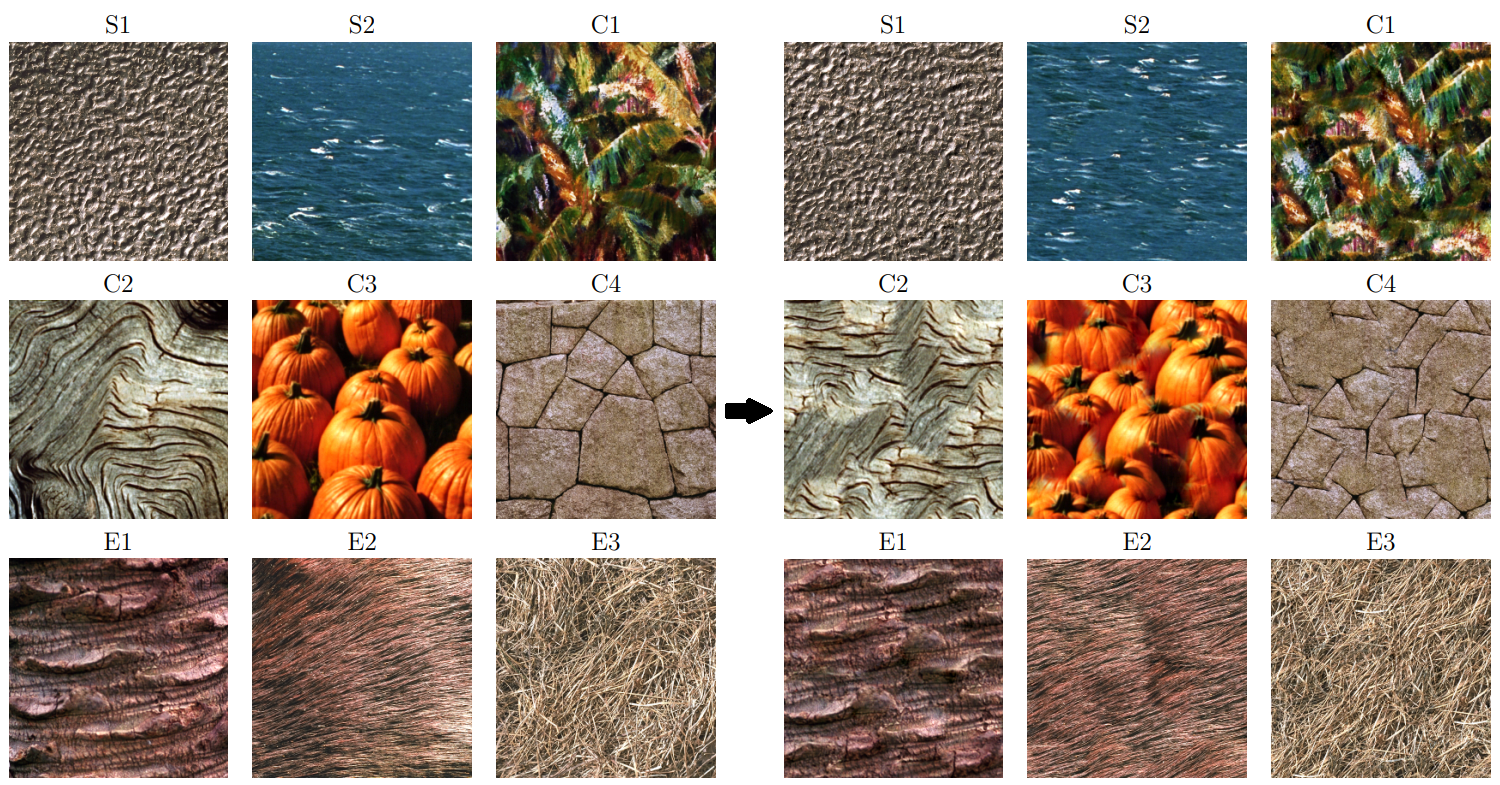
\includegraphics[width=1\textwidth, angle=0]{images/texsynth_input_output.png}
\caption{Output images for Patchwork texture synthesis \cite{harrison2002patchwork}}
\label{fig:texSynth}
\end{figure}
In computer graphics, texture synthesis is the problem of generating an output image that is bigger than the input image while resembling it. Most techniques solving this problem aim at having high similarity of patterns which are sub-images of small sizes (e.g. 5x5 pixels). It is worth mentioning that similarity, in most cases, is based on the Euclidean distance of pixel colors, whereas in the case of the WFC, patterns have to be an exact match. \cite{Smith}
The requirement of exact match of patterns allows for much wider use of the WFC than other typical texture synthesis tools, as with little adjustments users can easily define key features of the output image. \cite{GraphBased}
\begin{figure}[H]
\centering
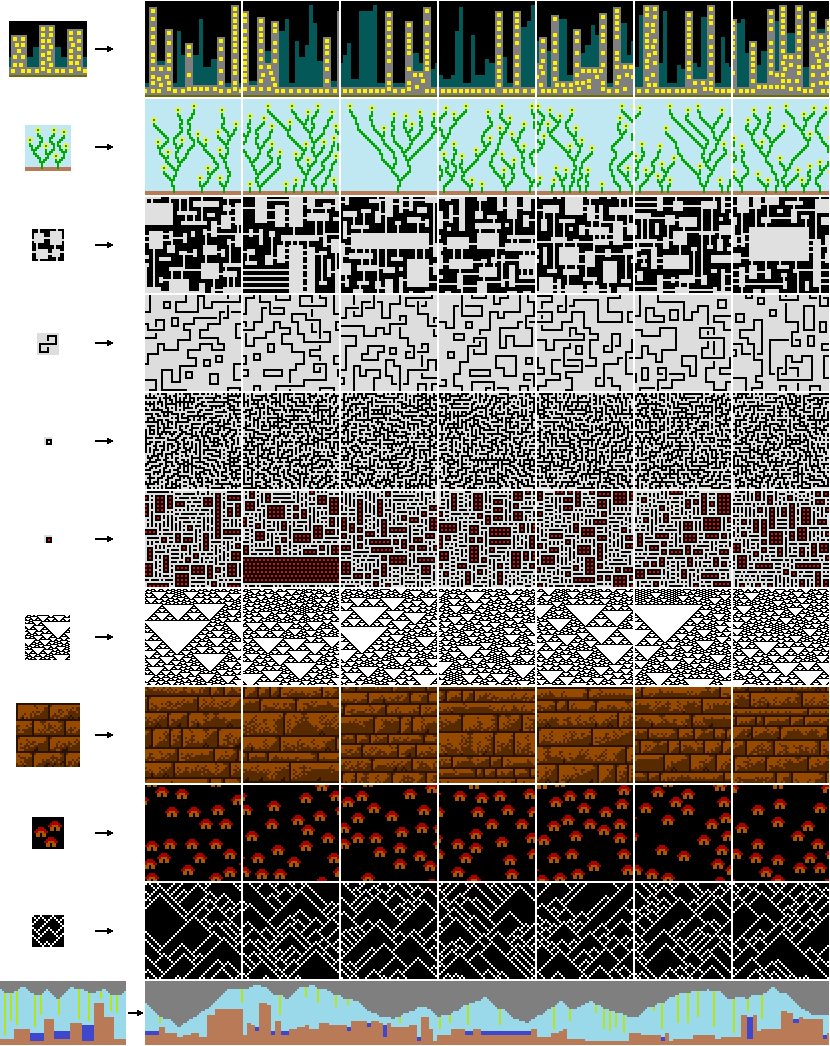
\includegraphics[width=1\textwidth, angle=0]{images/wfc.png}
\caption{Examples of inputs and outputs of the WFC algorithm \cite{MaximGumin}}
\label{fig:wfc}
\end{figure}
As stated by Maxim Gumin, the WFC tends to be slower than P. F. Harrison's texture synthesis algorithm (examples see Figure \ref{fig:texSynth}), but strict relation in which patterns have to be in images produced by the WFC, allows for capturing long correlations like a pattern of bricks, greenery or abstract shapes with a pixel perfect precision, which makes it the perfect candidate to use with pixel art and for level generation. See Figure \ref{fig:wfc}. \cite{MaximGumin}


\section{Constraint Solving Algorithms}
\begin{figure}[H]
\centering
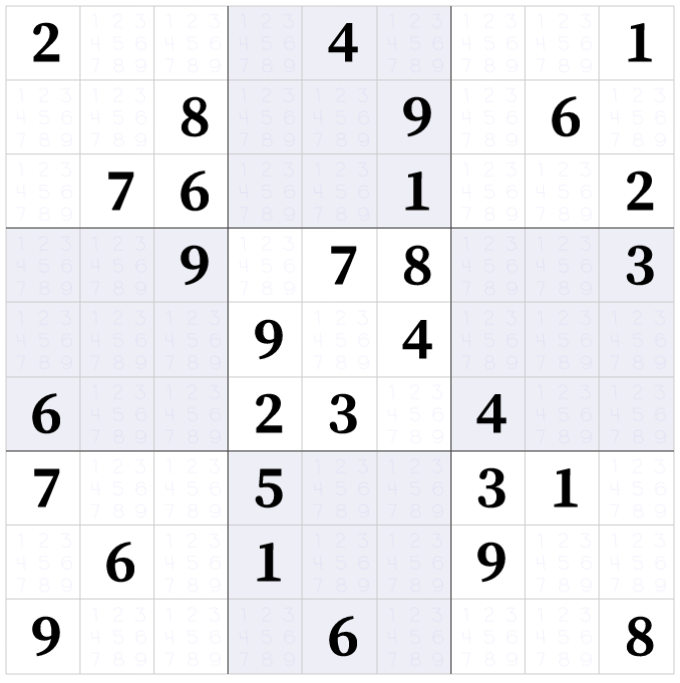
\includegraphics[width=1\textwidth, angle=0]{images/sudoku.png}
\caption{Example Sudoku problem \cite{sudoku}}
\label{fig:sudoku}
\end{figure}
Constraint satisfaction problems (CSPs) are typically defined in terms of decision variables and values. An example of it might be the Sudoku game, in which each location on the grid is a variable, and values come from a set of digits. The goal of an algorithm solving this kind of problems is to find a total assignment (each variable has an assigned value), that does not violate any constraints.

The WFC algorithm constructs the solution image by assigning values from a discrete set of unique local patterns from the input image. \cite{Smith} The key observation is that Maxim Gumin`s algorithm being a CSP solver means that each iteration (every step of the algorithm that assigns a value to the variable) produces a new valid problem. This can be used to guide algorithm by pre-assigning some variables, as partially solved CSP is still proper input for any solver (as long as partial assignment does not violate constraints).


\section{Procedural Content Generation}
PCG (procedural content generation) is a powerful tool wherever a high or countless amount of content is required, as it can reduce the resources spent on new assets by generating them based on those already manually created by artists or creating them entirely based on rules predefined in the algorithm. An important factor in deciding when to use the PCG is the cost of preparing the algorithm compared with the cost of manually making all assets. In the case of products that require a countless amount of assets, the PCG is the only option and has to be a highly controlled process. The upfront cost of using the PCG comes from choosing a well-fitted method, parameter tuning, profoundly understanding the design, and knowing how to encode it.


From the game development point of view, two types of the PCG can be distinguished. An offline variant is used for creating assets during development. It does not have to produce output in real-time and its output can be checked by artists before being used in the final product. On the other hand, the online algorithm is used in the final application runtime. It has to work in real-time and produce its output in an acceptable time. Artists can not check algorithm outputs, so it has to be highly controllable and fine-tuned during the development phase. \cite{DesignLevelConstraints}


WFC algorithm's main advantages in PCG are ease of use, as basic results can be achieved by tuning input image only, high controllability, as strict neighbor relations can guarantee the generation of playable content. It can be easily extended by adding additional rules like density, total count, and distance on top of neighbor relations. \cite{Smith, DesignLevelConstraints}



\chapter{WFC Applications}
\label{chapter2}
\section{Level Generation}
\begin{figure}[H]
\centering
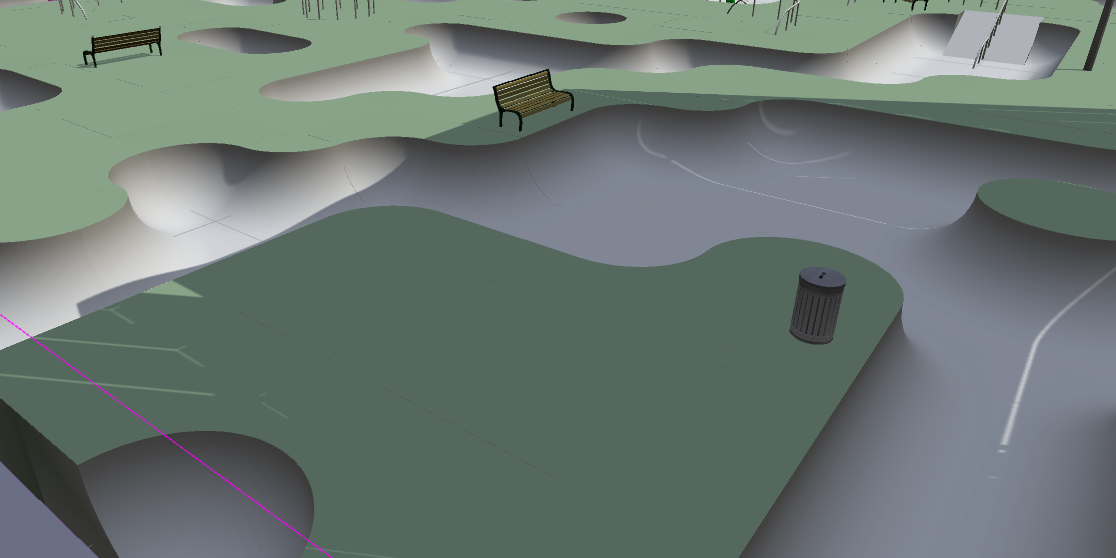
\includegraphics[width=1\textwidth, angle=0]{images/skater.png}
\caption{Proc Skater - the first game in which WFC was used for level generation \cite{skater}}
\label{fig:skater}
\end{figure}
The WFC algorithm appeared in a game for the first time during the ProcJam event in the form of a submission from Joseph Parker, Ryan Johns, and Oscar Morante - Proc Skater game. As stated by Joseph Parker, he has “never been this excited about an algorithm!”. In the case of their game, use of the WFC ensured smooth traversability of the level thanks to exact pattern matching.
\break\break\break\break\break

 Oskar Stålberg is another game developer who participated in the popularization of the WFC algorithm by creating a small demo web application\footnote{\url{http://oskarstalberg.com/game/wave/wave.html}}. He was one of the first to generalize WFC for other shapes and 3D meshes\footnote{\url{https://twitter.com/OskSta/status/784847588893814785}}. Oskar Stålberg also contributed by adding backtracking and bitwise operations as performance improvements. \cite{Smith} More about backtracking can be found in section \ref{backtracking}.


\section{Solving CSPs}
\begin{figure}[H]
\centering
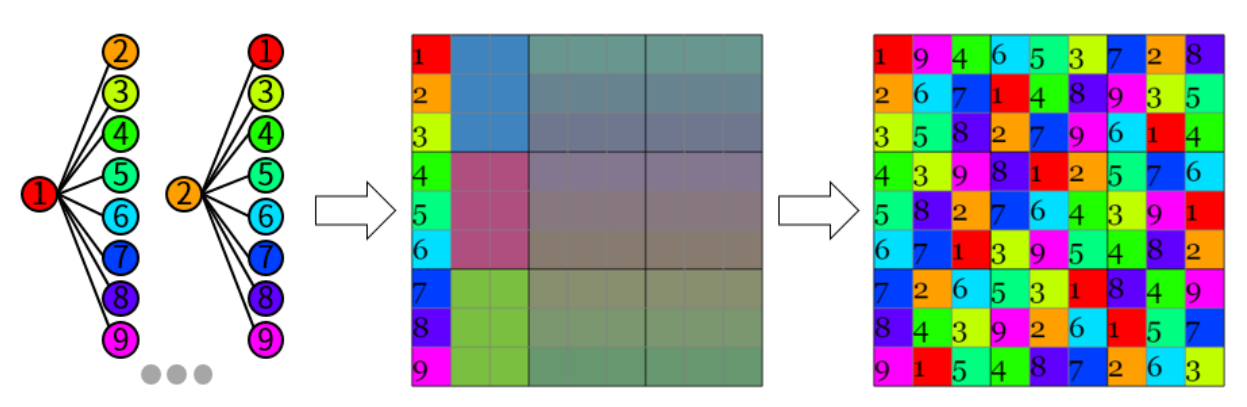
\includegraphics[width=1\textwidth, angle=0]{images/sudoku_solver.png}
\caption{Sudoku allowed neighbors, initial state, puzzle solved using graph-based WFC \cite{GraphBased}}
\label{fig:sudoku_solver}
\end{figure}
The WFC algorithm can be used to solve CSPs if properly modified to fit the domain. An example would be solving the Sudoku game with WFC generalized for graphs which was done as a part of "Automatic Generation of Game Content using a Graph-based Wave Function Collapse Algorithm" \cite{GraphBased}. This paper focused on generalizing WFC by allowing each element to have a variable amount of neighbors but with the drawback of not distinguishing directions\footnote{the original WFC uses neighbor relations like "A is left neighbor of B" whereas, in the  case of the graph-based solution, we only know that "A is neighbor of B"}. For solving the Sudoku, game rules can be formulated to fit this model - each variable has 20 neighbors. The Figure \ref{fig:sudoku_neighbors} represents neighbors of a blue variable.
\begin{figure}[H]
\centering
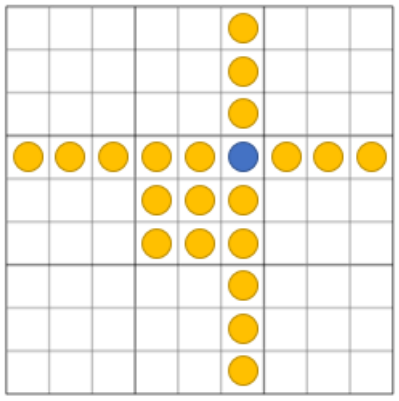
\includegraphics[width=0.5\textwidth, angle=0]{images/sudoku_neighbors.png}
\caption{blue represents selected Sudoku grid element, yellow represents its neighbors}
\label{fig:sudoku_neighbors}
\end{figure}
Backtracking had to be added to the WFC for it to be able to produce solutions for Sudoku puzzles, as contradictions were common due to very strict rules. Even with backtracking, the WFC is not performing well as a CSP solver, but on the other hand, it can deduce the rules of the problem on its own. \cite{GraphBased}
\begin{figure}[H]
\centering
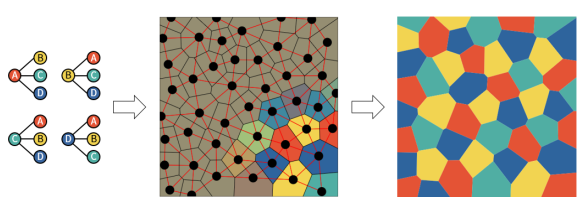
\includegraphics[width=1\textwidth, angle=0]{images/fourcolours.png}
\caption{Four Colours Problem being solved by WFC \cite{GraphBased}}
\label{fig:fourcolours}
\end{figure}
The same version of the WFC algorithm solves the four colors problem, thanks to it being directly representable as a graph. Algorithm was able to solve this CSP with basic rules of the four colors problem which it could deduce from the example solution, without any additional heuristics. \cite{GraphBased} The Figure \ref{fig:fourcolours} represents the process of solving the four colors problem with the WFC algorithm.


\section{Writing Poetry}
\begin{figure}[H]
\centering
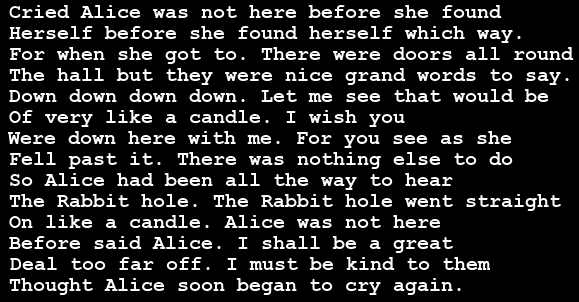
\includegraphics[width=1\textwidth, angle=0]{images/poem.png}
\caption{Poem written by Martin O’Leary WFC inspired algorithm  \cite{wfcpoem}}
\label{fig:poem}
\end{figure}
One of the most unexpected forms of the content generated with the WFC algorithm is poetry. Martin O'Leary, inspired by Maxim Gumin's work, decided to use the WFC algorithm to generate poetry with rhyme and meter constraints. Rhyme and meter constraints are long-distance constraints, as opposed to the short-distance constraints originally used in the WFC algorithm. The WFC algorithm creates tiles from syllables. The results of using the WFC algorithm to generate poetry with rhyme and meter constraints can be seen in Figure \ref{fig:poem}. \cite{Smith, wfcpoem}


\chapter{The WFC Algorithm}
\label{chapter3}
\section{Pseudo Code}
\begin{enumerate}
    \item Read the input bitmap and count NxN patterns.
    \item Create an array with the dimensions of the output (wave). Each element of this array represents a state of an NxN region in the output. A state of an NxN region in the output is a superposition of NxN patterns from the input with Boolean coefficients. The false coefficient means that the corresponding pattern is forbidden. The true coefficient means that the corresponding pattern is not yet banned. This means that the color of each pixel in the output is the average of colors of not forbidden patterns.
    \item Initialize the wave in the completely unobserved state, in other words with all the Boolean coefficients being true.
    \item \label{loop}Repeat the following steps:
    \begin{enumerate}
        \item Observation:
Find a wave element with minimal nonzero entropy. If there are no elements with minimal nonzero entropy (in other words if all elements have zero or undefined entropy), break the cycle (\ref{loop}) and proceed to step (\ref{final_step}). If there are some elements, choose one at random and discard others.
        \item Propagation: propagate information gained on the previous observation step.
    \end{enumerate}
    \item \label{final_step}By now all the wave elements are either in a completely observed state (all the coefficients except one being zero) or in a contradictory state (all the coefficients being zero). In the first case return the output. In the second case, the algorithm finishes without producing any result.
\end{enumerate}
\cite{MaximGumin}

\section{Deducing Rules}
Patterns of size NxN are taken from the input image. Additional patterns can be generated from symmetries and rotations of the original patterns. Every NxN part of the output image should belong to patterns deduced from the input image, making the WFC useful in scenarios where pixel-perfect precision is required, such as level generation or pixel art. \cite{MaximGumin}


\section{Observation}
The observation phase in the WFC algorithm handles two tasks: it finds the lowest non-zero entropy\footnote{variable that can be assigned the least values but is not yet assigned} and collapses it\footnote{assigns value to the variable}.
In the original WFC implementation, finding the lowest non-zero entropy is done by simply searching through all variables and looking for the one with the least possible assignments. \cite{MaximGumin} This approach is sufficient for small bitmaps. For larger data sets, this process would benefit from introducing a priority queue that supports the decrease key operation.
 More information about this improvement can be found in sections \ref{fibheap} and \ref{prioritybuckets}.

\section{Propagation}
The propagation phase in the WFC algorithm handles updating possible assignments for each variable. Possible assignments must be based on constraints given by the possible values of neighbors. The set of possible values is the intersection of allowed values from each neighbor. The allowed values from every neighbor are the union of possible values for each legal assignment. Implementing possible values as some kind of a set is quite intuitive, but it is important to note that many union and intersection operations are performed.

The original implementation uses Boolean vectors of domain length, where each value represents whether the value is legal. Maxim Gumin wrote his algorithm in in C\#, where Boolean vectors are specialized to store Boolean values in a single bit\footnote{Boolean vector specialization in C\# \url{https://learn.microsoft.com/en-us/cpp/standard-library/vector-bool-class?view=msvc-170}}. However, it is not specified by the language if there are any optimizations for a series of logic operations. Furthermore, many programming languages do not have specialized Boolean vectors. More about data structure for storing possible variable assignments can be found in the section \ref{bitwise}.

\break\break
The simplest solution would be to update all possible variable assignments as long as the system is unstable. However, it is important to note that updating a variable might require updating each of its neighboring variables. Updates of variables happen both due to the observation and propagation phases. This makes the propagation phase quite expensive and an obvious candidate for optimization. The stack can be used to keep track of elements that require updates, as the author of the WFC algorithm did in his implementation. Similarly, a queue can be used. A comparison of these two solutions can be found in the section \ref{stack_vs_queue}.


\section{Backtracking}
\label{backtracking}
In the original WFC implementation, there is no backtracking, if a contradiction is detected, the algorithm will retry the whole generation process. Isaac Karth and Adam M. Smith showed in their work that the contradiction rate depends on how strict the rules for assignments are. In simple examples shown by Maxim Gumin, the contradiction rate is low enough not to use backtracking, but for larger scale problems with more heuristics, the backtracking becomes crucial for the WFC to work correctly.
\cite{Smith}



\chapter{Performance Comparison}
\label{chapter4}
For performance comparison purposes, we have created five versions of the WFC algorithm in the Rust programming language. From a performance perspective, the deducing rules phase is not interesting and as a result, is skipped. Instead, the input to the algorithm is a tile set with constraints and a tilemap to fill (it can be partially assigned). We have been running benchmarks on the tile set with relaxed restrictions\footnote{each tile has a high number of allowed neighbors}. To eliminate contradictions, the tile set contains a tile that can be a neighbor of any other tile, making the benchmarks more stable.


To validate the correctness of all solutions, we have written tests to verify that the output follows the given rules. It is important to note that for probabilistic algorithms, these tests must be run multiple times to ensure correctness.


We utilized the Criterion\footnote{A statistics-driven micro-benchmarking library written in Rust \url{https://docs.rs/criterion/latest/criterion/}} library for benchmarking all implementations and Perf\footnote{about perf \url{https://perf.wiki.kernel.org/index.php/Main_Page}} with Flamegraph\footnote{cargo flamegraph - the Flamegraph generator written in rust \url{https://github.com/flamegraph-rs/flamegraph}} for profiling.

During code analysis, we consider the size of the problem (\( n \)) and tile set size (\( m \)). Size of the problem is calculated as \( m = xyz\) where \(x\), \(y\), and \(z\) represent the dimensions of the problem to be solved.

\break\break\break
\section{Boolean Vector As Representation Of States}
\subsection{Code Analysis}
This implementation involves representing possible assignments with Boolean vectors.  For each neighbor, the algorithm calculates the union of the allowed neighbors for each possible assignment.  The intersection of the results from all neighbors gives the current possible assignments for that variable.





\begin{figure}
\begin{minted}{rust}
vec![
...
solution.get(x, y, z + 1) //front neighbor
        .iter()
        .zip(0..u8::MAX)
        .filter_map(|(b, idx)| match b{true => Some(idx), false => None})
        .map(|idx| rules[idx as usize].back()) //allowed back neighbors
        .fold(vec![false;u8::MAX as usize],
              |acc:Vec<bool>, b| acc.iter()
                                    .zip(b)
                                    .map(|(&a,&b)| a||b)
                                    .collect())
...
];

\end{minted}
\caption{legal moves - union of allowed neighbors of each possible assignment (calculated for one of six neighbors)}
\label{fig:legal-union}
\end{figure}

\begin{figure}
\begin{minted}{rust}
...
w.iter() //iterate over allowed neighbors from all directions
 .fold(vec![true; u8::MAX as usize],
       |acc, x| acc.iter()
                   .zip(x)
                   .map(|(&a,&b)| a && b)
                   .collect())
\end{minted}
\caption{legal moves - intersection calculated from all directions}
\label{fig:legal-intersection}
\end{figure}

There are at most \( m \) Boolean vectors of size \( m \) to merge (union). This operation must be performed for each of the six directions in a 3D grid of cubes (as shown in code fragment Figure \ref{fig:legal-union})

The algorithm performs the intersection of the six allowed neighbors sets (as shown in code fragment Figure \ref{fig:legal-intersection}).

Updating possible assignments takes the following steps:
\begin{enumerate}
    \item getting rules for each neighbor \(\mathcal{O}(6m) = \mathcal{O}(m)\)
    \item union for each neighbor \(\mathcal{O}(6m^2) = \mathcal{O}(m^2)\)
    \item intersection \(\mathcal{O}(6m) = \mathcal{O}(m)\)
\end{enumerate}
Total \(\mathcal{O}(12m + 6m^2) = \mathcal{O}(m+m^2)\).

This operation should be performed at most \(6nm\) times, as it is only performed if the number of possible assignments changes for one of the variables. The number of possible assignments for one variable can decrease at most \(m\) times. Whenever one variable updates, there are six neighbors that must be checked for updates.

This variant of the algorithm does not keep track of variables that require updating, which causes it to perform the variable update \(n^2m\) times, as every time, something needs to be updated, the algorithm updates all variables.

The time complexity for the propagation phase, which is responsible for updating the possible assignments, is \(\mathcal{O}(n^2(12m^2 + 6m^3)) = \mathcal{O}(n^2(m^2+m^3))\).

\begin{figure}
\begin{minted}{rust}
fn find_minimal(solution: &Vec3D<Vec<bool>>) -> Option<(usize,usize,usize, Vec<bool>)>
{
    PosIter3D::new(solution)
    .map(|(x,y,z)| Some((x, y, z, solution.get(x, y, z))))
    .fold(None, |acc, x| {
        match acc
        {
            Some(a) => {
                let x = x.unwrap();
                let next_len = x.3.iter().filter(|&&x|x).count();
                let this_len = a.3.iter().filter(|&&x|x).count();
                if  next_len > 1 && next_len < this_len
                {
                    Some(x)
                }
                else
                {
                    Some(a)
                }
            },
            None =>
            {
                let x = x.unwrap();
                let next_len = x.3.iter().filter(|&&x|x).count();
                if next_len > 1
                {
                    Some(x)
                }
                else
                {
                    None
                }
            }
        }
    })
}
\end{minted}
\caption{find min}
\label{fig:observe-findmin}
\end{figure}

During the observation phase, the WFC algorithm finds the variable with the least possible assignments and assigns a value selected at random. The complexity of finding the minimum value is \(\mathcal{O}(nm)\), as it simply scans all variables and counts their possible assignments (the code for finding the minimum is shown in Figure \ref{fig:observe-findmin}). The algorithm performs at most \(n\) observations.


Time complexity of this WFC variant is

\(\mathcal{O}(mn^2 + n^2(12m^2 + 6m^3)) = \mathcal{O}(n^2(m + m^2 + m^3))\).


\subsection{Performance}
\begin{figure}[H]
\centering
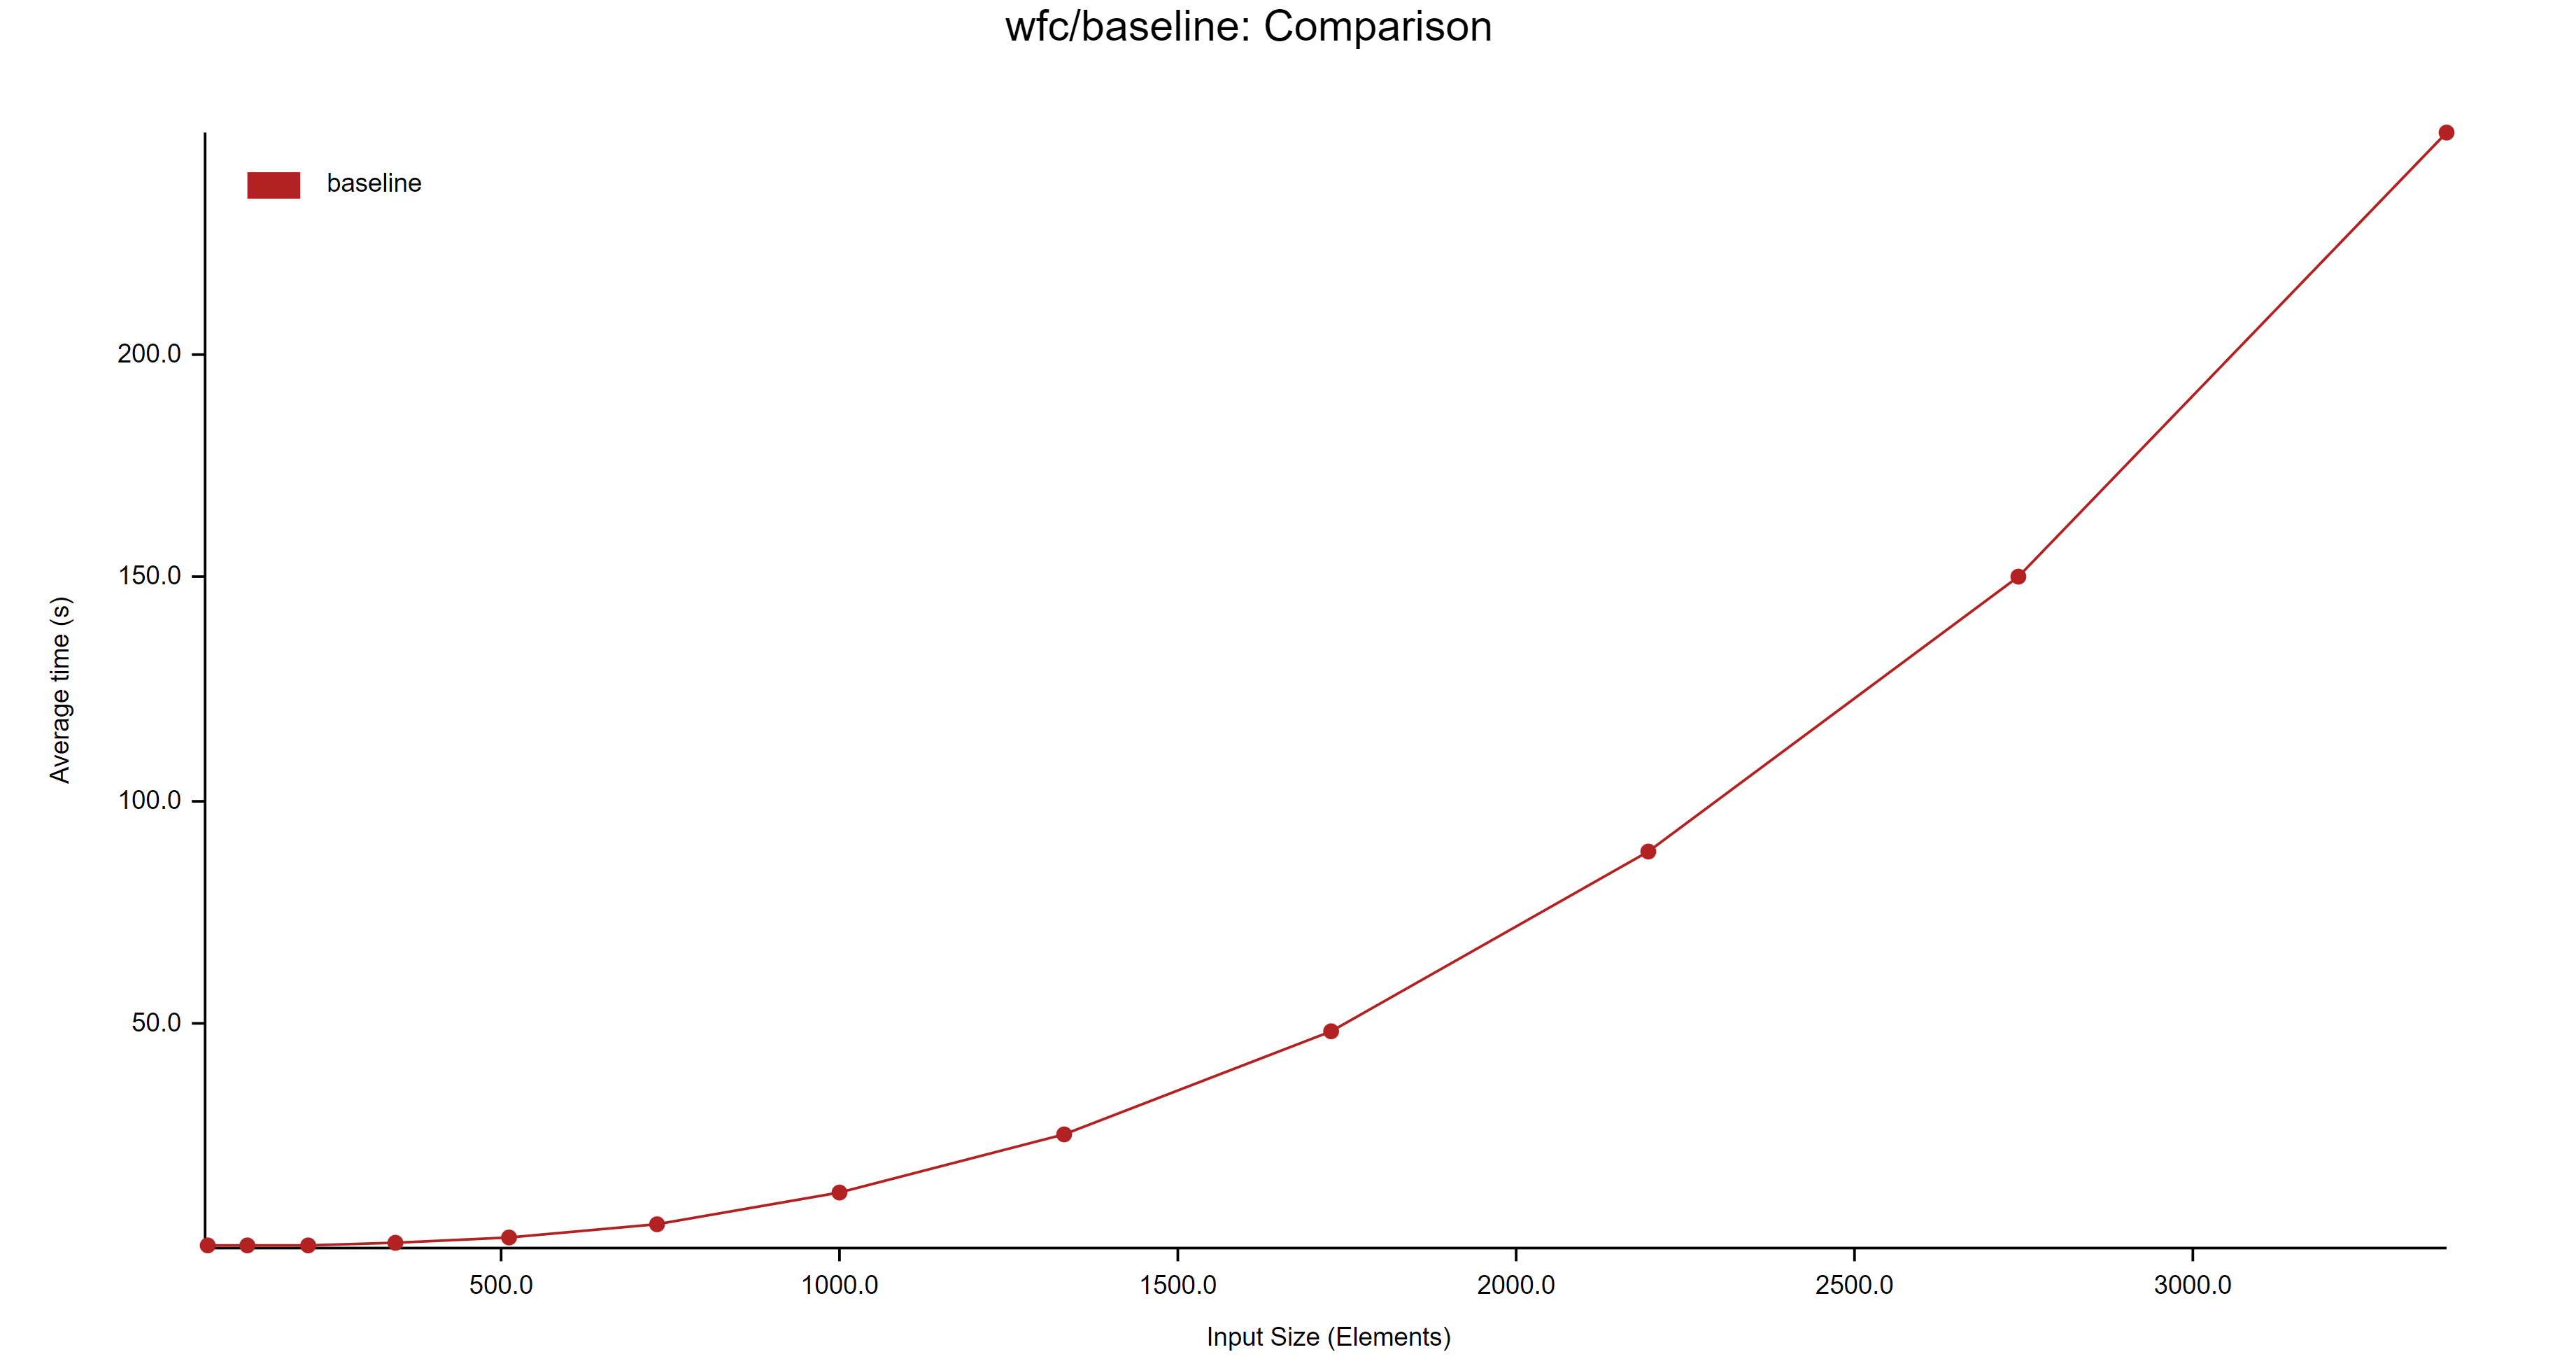
\includegraphics[width=1\textwidth, angle=0]{images/baseline_performance.png}
\caption{performance of the baseline implementation of WFC}
\label{fig:baseline_performance}
\end{figure}

From benchmarks we can observe polynomial nature of this implementation (Figure \ref{fig:baseline_performance}. For the relatively small problem (\(m=256\) and \(n=3375\)), algorithm takes 250 seconds on average. From the flame graph (see Figure \ref{fig:baseline_flamegraph}) we can see that most of the time is spent in the propagation phase (\(99\%\)).

Benchmark results match with the static code analysis, as we can see similar characteristics of the theoretical complexity and measured running time. Additionally, high disproportion in complexity of the propagation and observation phases can be observed both on the flamegraph and in the analysis.

\begin{table}[]
\centering
\begin{tabular}{@{}l|r|r|r|r|@{}}
\cmidrule(l){2-5}
                                 & \multicolumn{1}{c|}{Lower bound} & \multicolumn{1}{c|}{Estimate} & \multicolumn{1}{c|}{Upper bound} & \multicolumn{1}{c|}{Units} \\ \midrule
\multicolumn{1}{|l|}{Throughput} & 13.42                            & 13.52                         & 13.65                            & elem/s                     \\ \midrule
\multicolumn{1}{|l|}{Mean}       & 247.23                           & 249.57                        & 251.53                           & s                          \\ \midrule
\multicolumn{1}{|l|}{Std. Dev.}  & 1.60                             & 3.69                          & 5.14                             & s                          \\ \midrule
\multicolumn{1}{|l|}{Median}     & 247.98                           & 249.95                        & 252.93                           & s                          \\ \bottomrule
\end{tabular}
\caption{baseline performance measured with \(m=256\) and \(n=3375\)}
\label{table:baseline}
\end{table}

\begin{figure}[H]
\centering
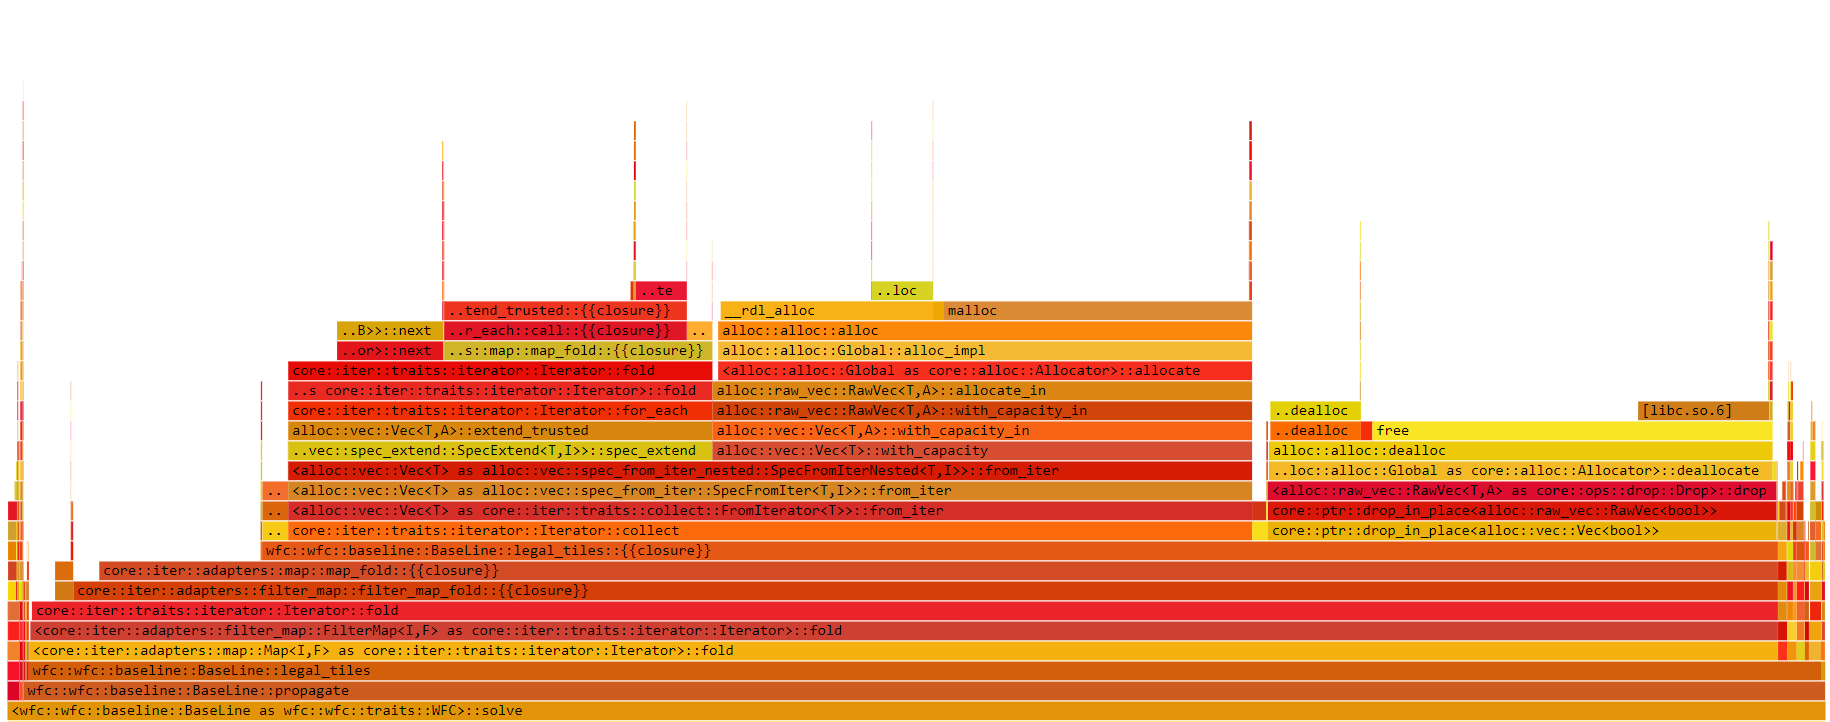
\includegraphics[width=1\textwidth, angle=0]{images/baseline_flamegraph.png}
\caption{performance of the baseline implementation of WFC}
\label{fig:baseline_flamegraph}
\end{figure}


\section{Keeping Track of Elements To Be Propagated Next}
\label{stack}
\begin{figure}[H]
\centering
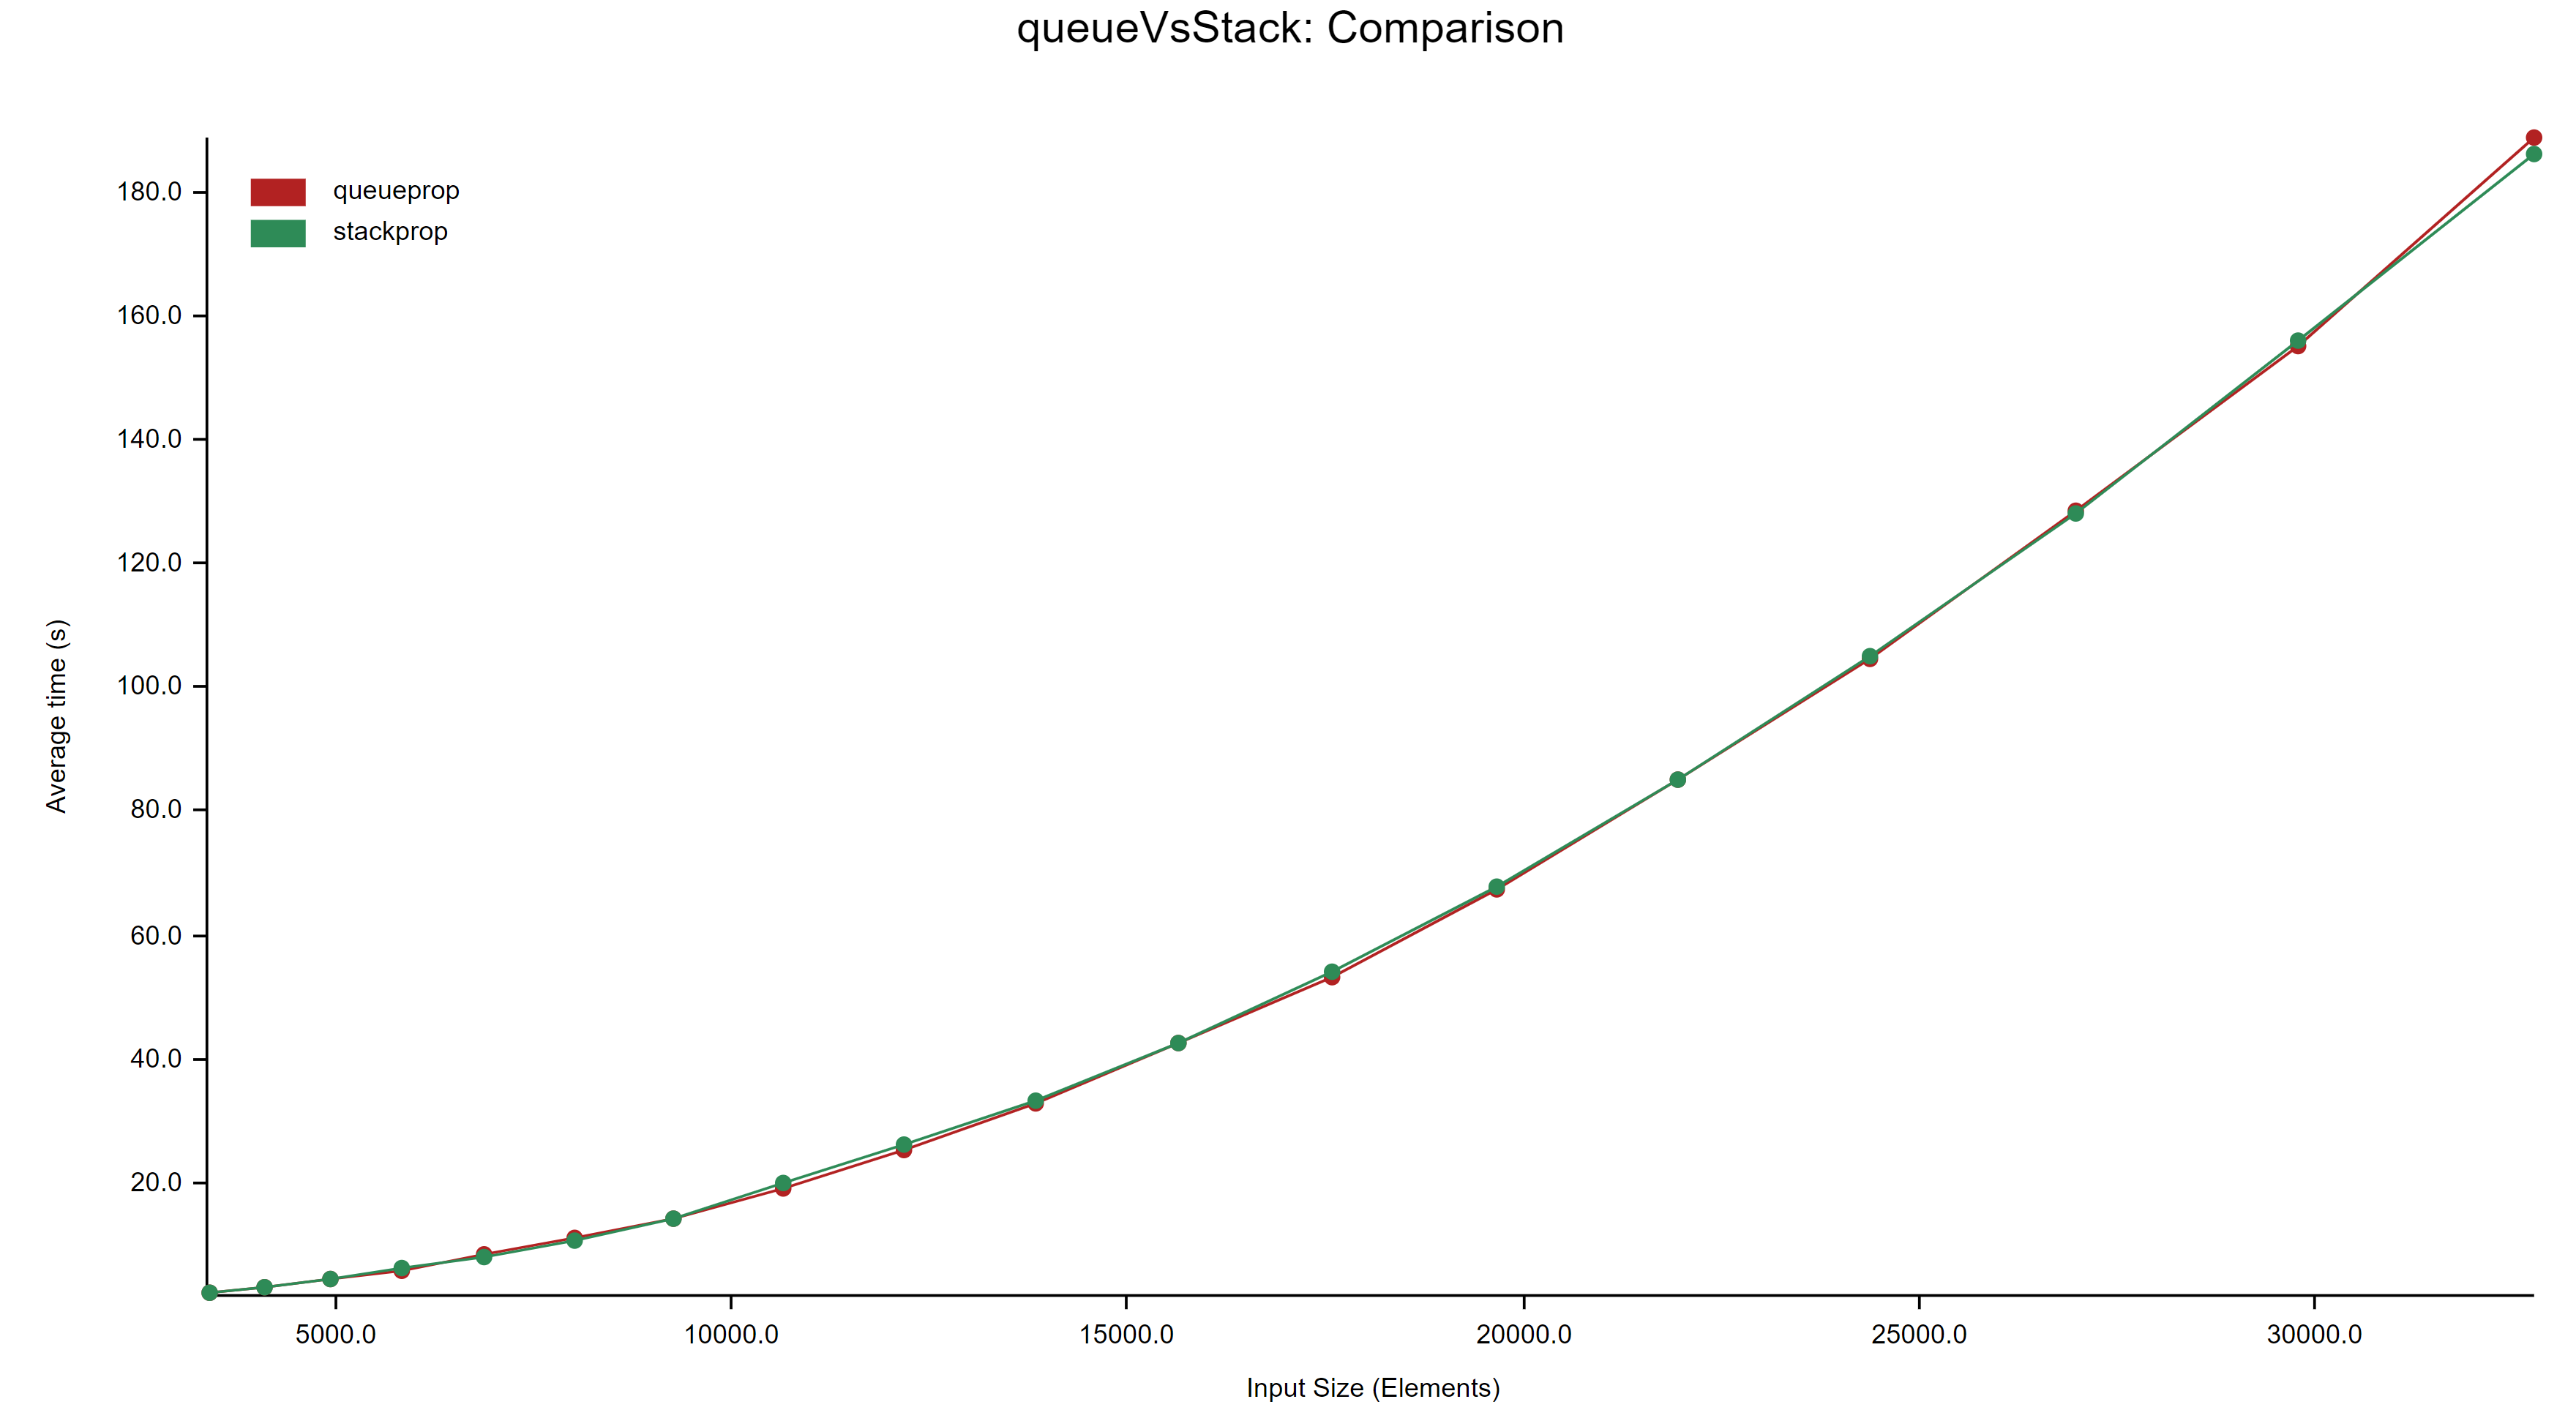
\includegraphics[width=1\textwidth, angle=0]{images/queue_vs_stack_performance.png}
\caption{performance of the variants using queue and stack}
\label{fig:queue_performance}
\end{figure}
\subsection{Code Analysis}
The only difference from the baseline implementation is the introduction of a structure for keeping track of all the elements that require updates. Maxim Gumin utilized a stack in his implementation, which allowed for a maximum of \(6nm\) updates, instead of \(n^2m\) in the baseline approach.

The time complexity of this variant is \(\mathcal{O}(mn^2 + n(72m^2 + 36m^3)) = \mathcal{O}(mn^2 + n(m^2 + m^3))\). This represents significant improvement, as usually \(m\) (domain size) tends to be relatively small. The propagation phase now operates in pseudo-linear time (linear if \(m\) can be considered constant).

\subsection{Performance}
\begin{table}[]
\centering
\begin{tabular}{@{}l|r|r|r|r|@{}}
\cmidrule(l){2-5}
                                 & \multicolumn{1}{c|}{Lower bound} & \multicolumn{1}{c|}{Estimate} & \multicolumn{1}{c|}{Upper bound} & \multicolumn{1}{c|}{Units} \\ \midrule
\multicolumn{1}{|l|}{Throughput} & 143.83                           & 145.15                        & 146.36                           & elem/s                     \\ \midrule
\multicolumn{1}{|l|}{Mean}       & 268.55                           & 270.78                        & 273.27                           & s                          \\ \midrule
\multicolumn{1}{|l|}{Std. Dev.}  & 1.92                             & 4.04                          & 5.03                             & s                          \\ \midrule
\multicolumn{1}{|l|}{Median}     & 267.06                           & 270.29                        & 273.56                           & s                          \\ \bottomrule
\end{tabular}
\caption{queue used for propagation performance measured with \(m=256\) and \(n=39304\)}
\label{table:queue}
\end{table}

By introducing a structure to keep track of elements that require updates, we significantly improved performance. On average, the algorithm takes 267 seconds to solve problems with \(n=39304\).

\begin{figure}[H]
\centering
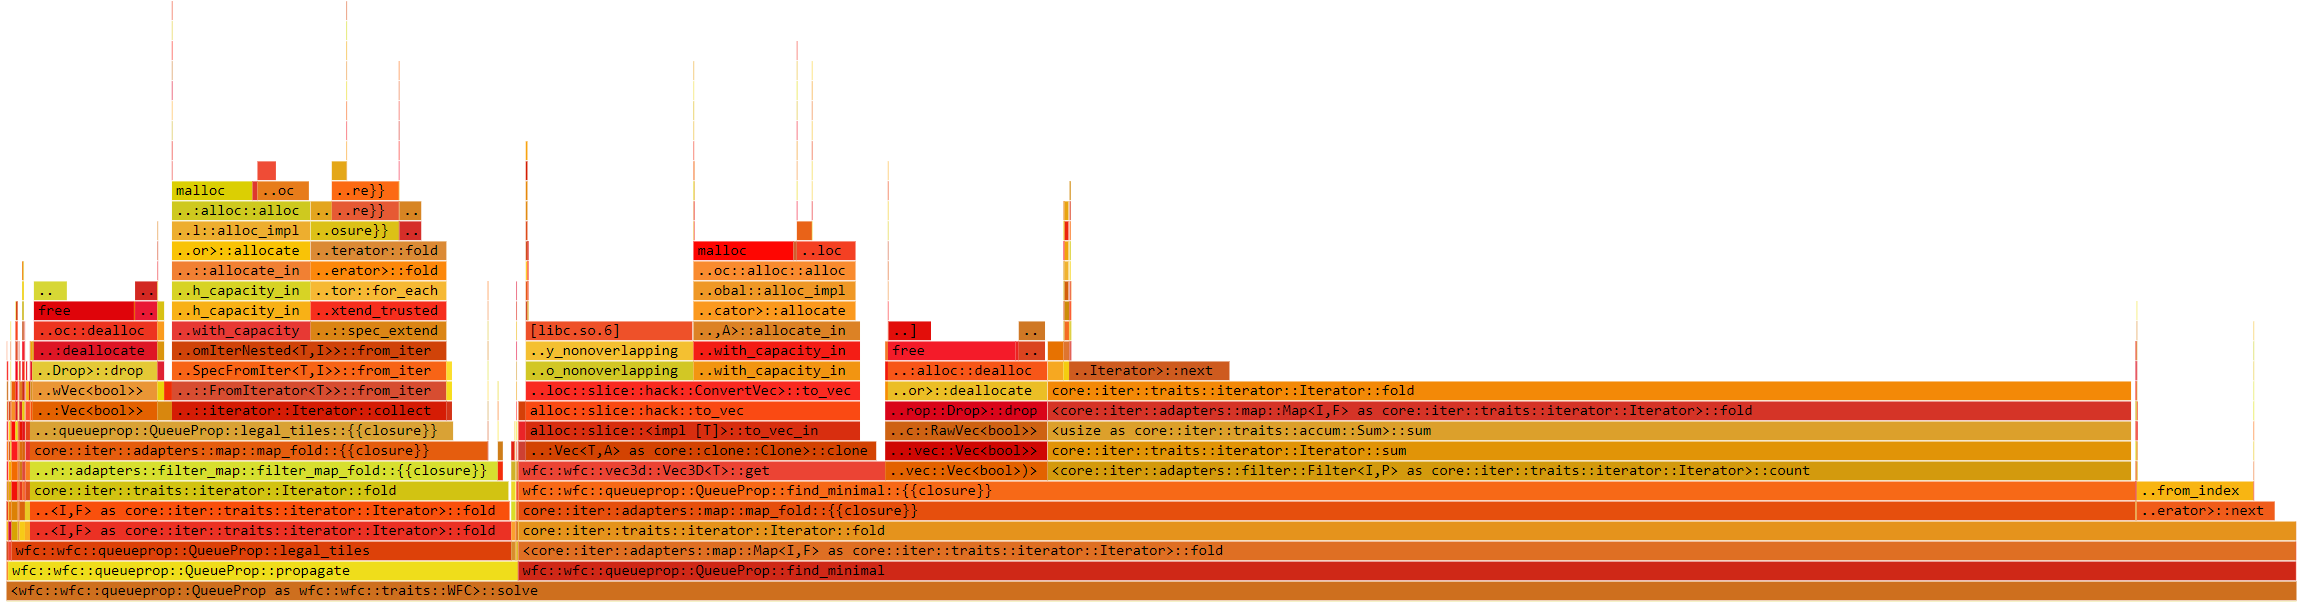
\includegraphics[width=1\textwidth, angle=0]{images/queueprop_flamegraph.png}
\caption{performance of the variant using queue}
\label{fig:queueprop_flamegraph}
\end{figure}

The flamegraph in Figure \ref{fig:queueprop_flamegraph} shows a greatly reduced ratio of time spent in the propagation phase. Propagation takes about \(22\%\) of the time.



\subsection{Stack vs Queue}
\begin{figure}[H]
\centering
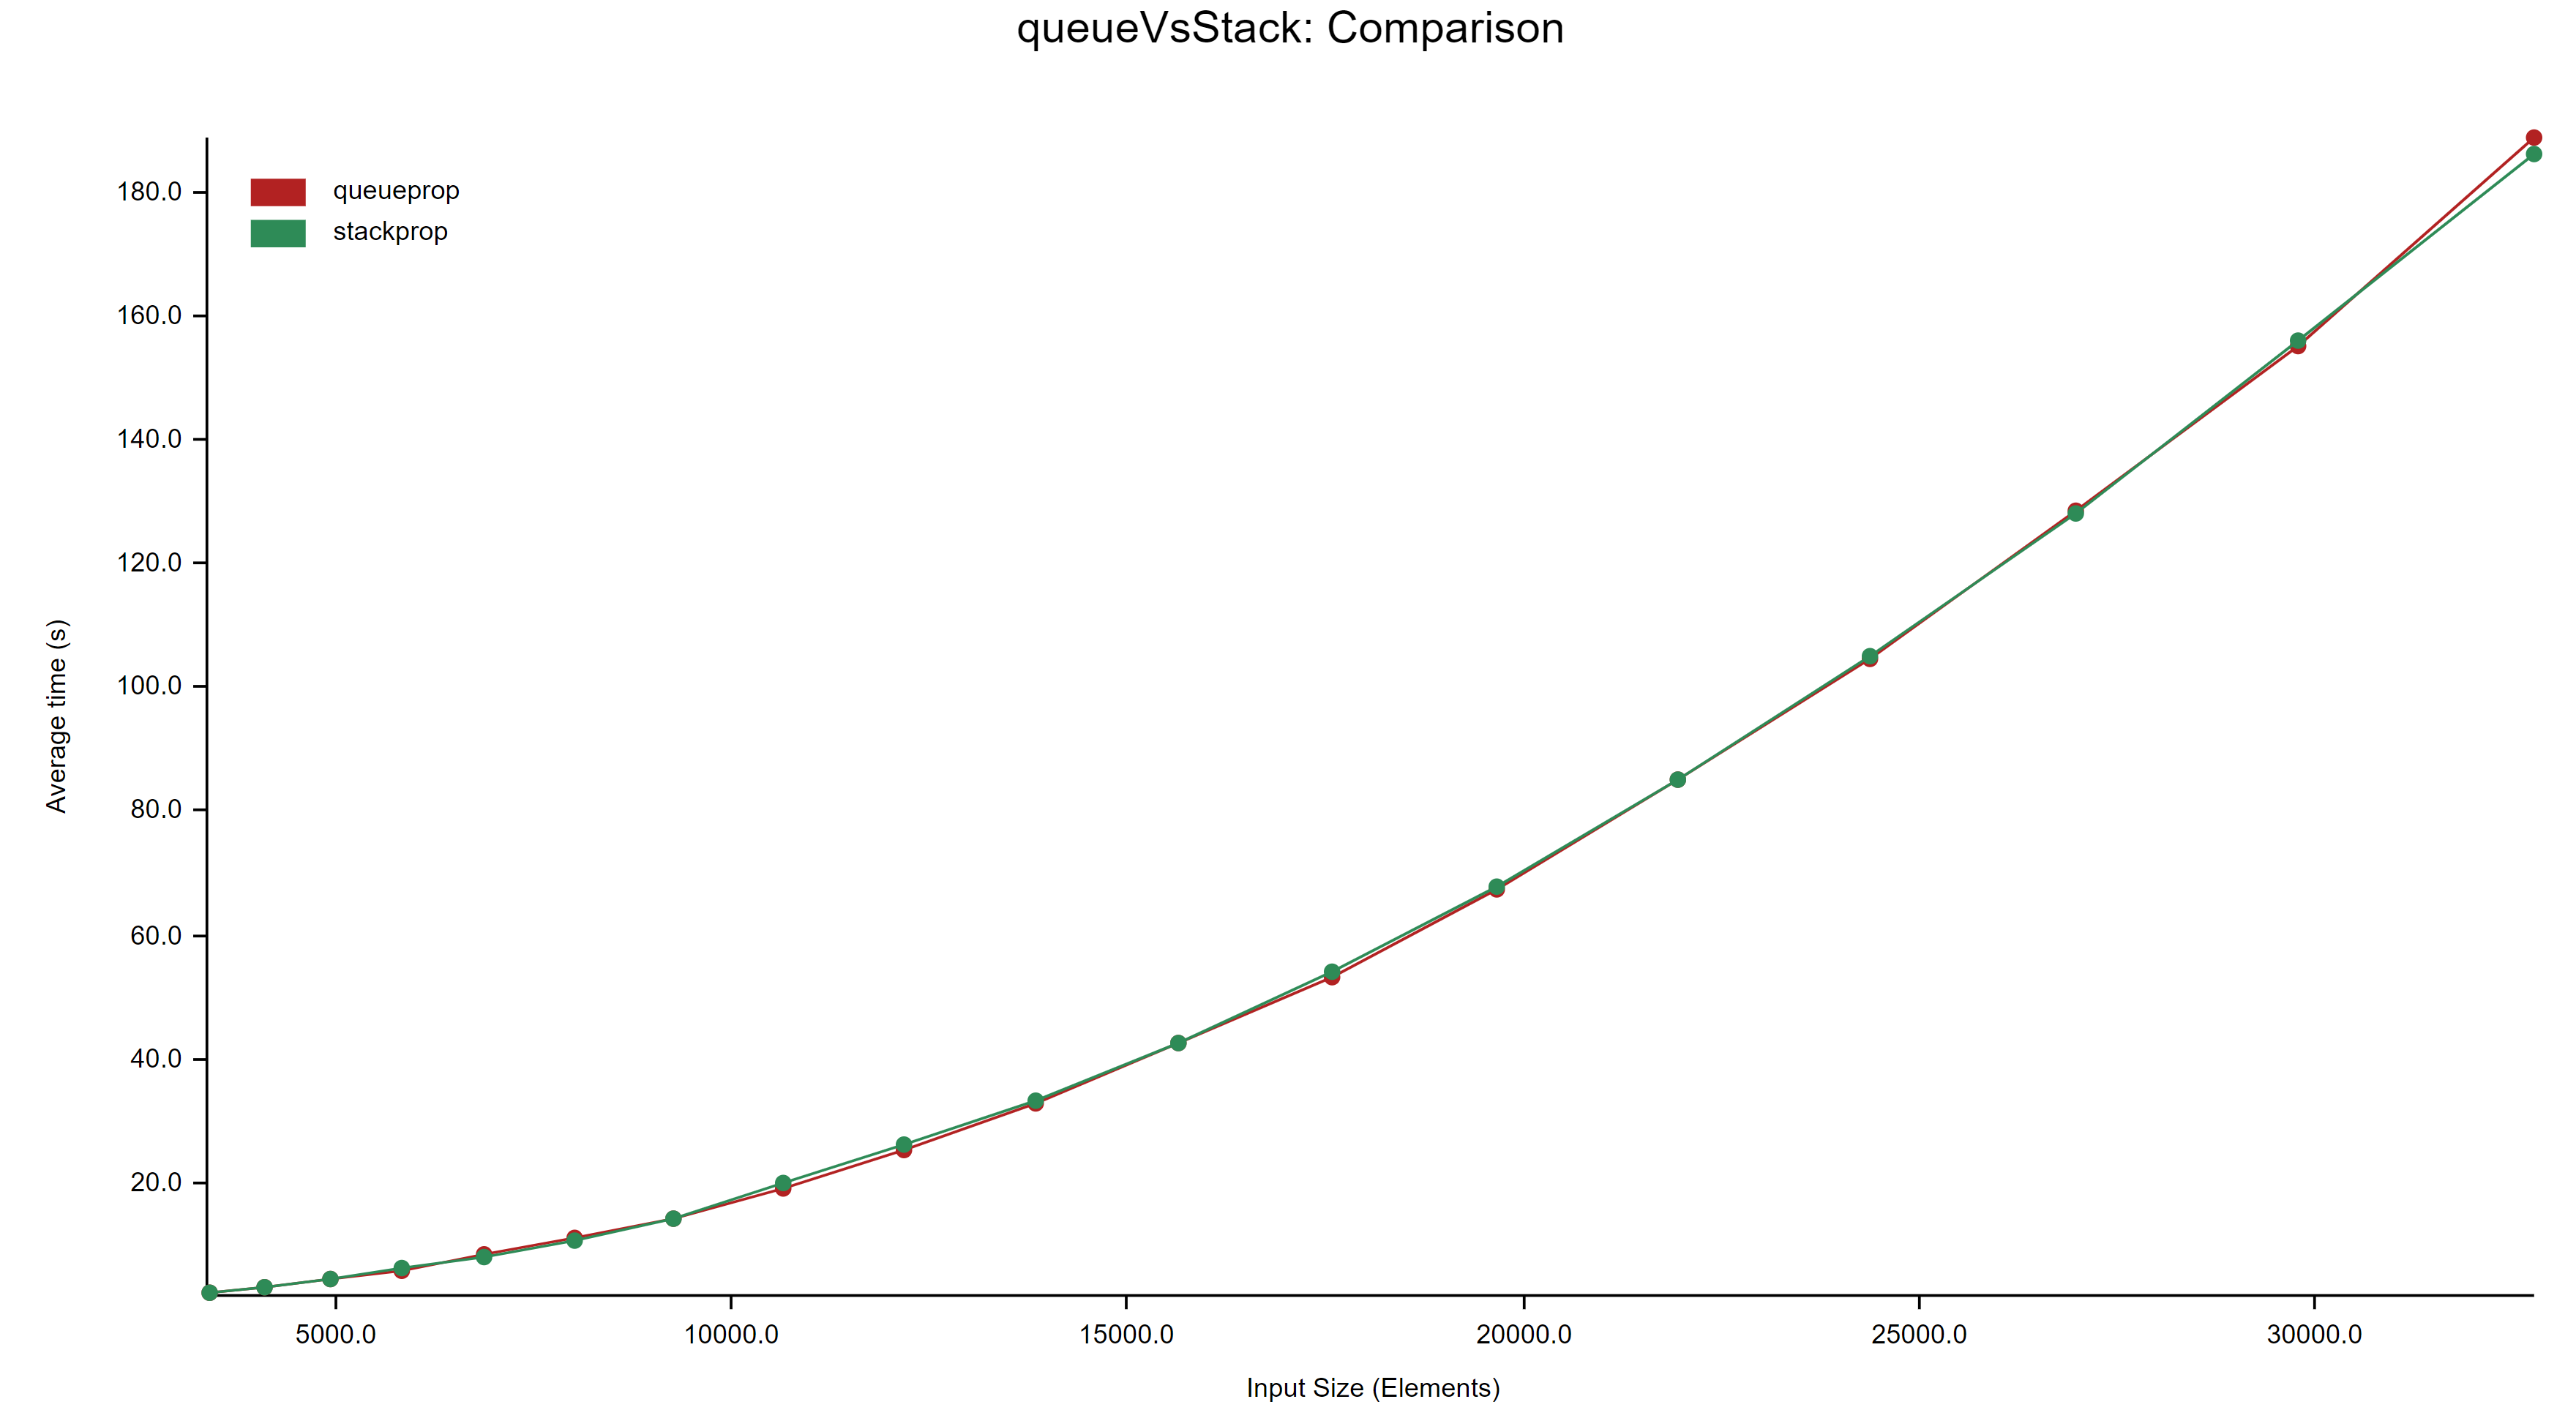
\includegraphics[width=1\textwidth, angle=0]{images/queue_vs_stack_performance.png}
\caption{performance of the variants using queue and stack}
\label{fig:stack_vs_queue}
\end{figure}
\label{stack_vs_queue}
The reason for testing both stack and queue is to evaluate the impact of the order of propagation on performance. Using queue results in propagation done in breadth-first search order, while using a stack results in depth first search order. This could have an impact on performance due to changes in locality. As shown in Figure \ref{fig:stack_vs_queue}, the difference in performance of those variants is insignificant.

To obtain a greater difference in queue and stack performance, it may be possible to improve spatial locality by aligning the array layout with traversal order. Currently, elements are stored in lexicographical order of their position, but the actual traversal order is determined by euclidean distance. The next item processed by the algorithm is most likely close in terms of euclidean distance to the previous element. Splitting the problem into cache friendly chunks, would reduce cache misses. More information about this idea can be found in section \ref{chunks}.


\section{Bitwise Operations And Bits As Representation For States}
\label{stack}
\begin{figure}[H]
\centering
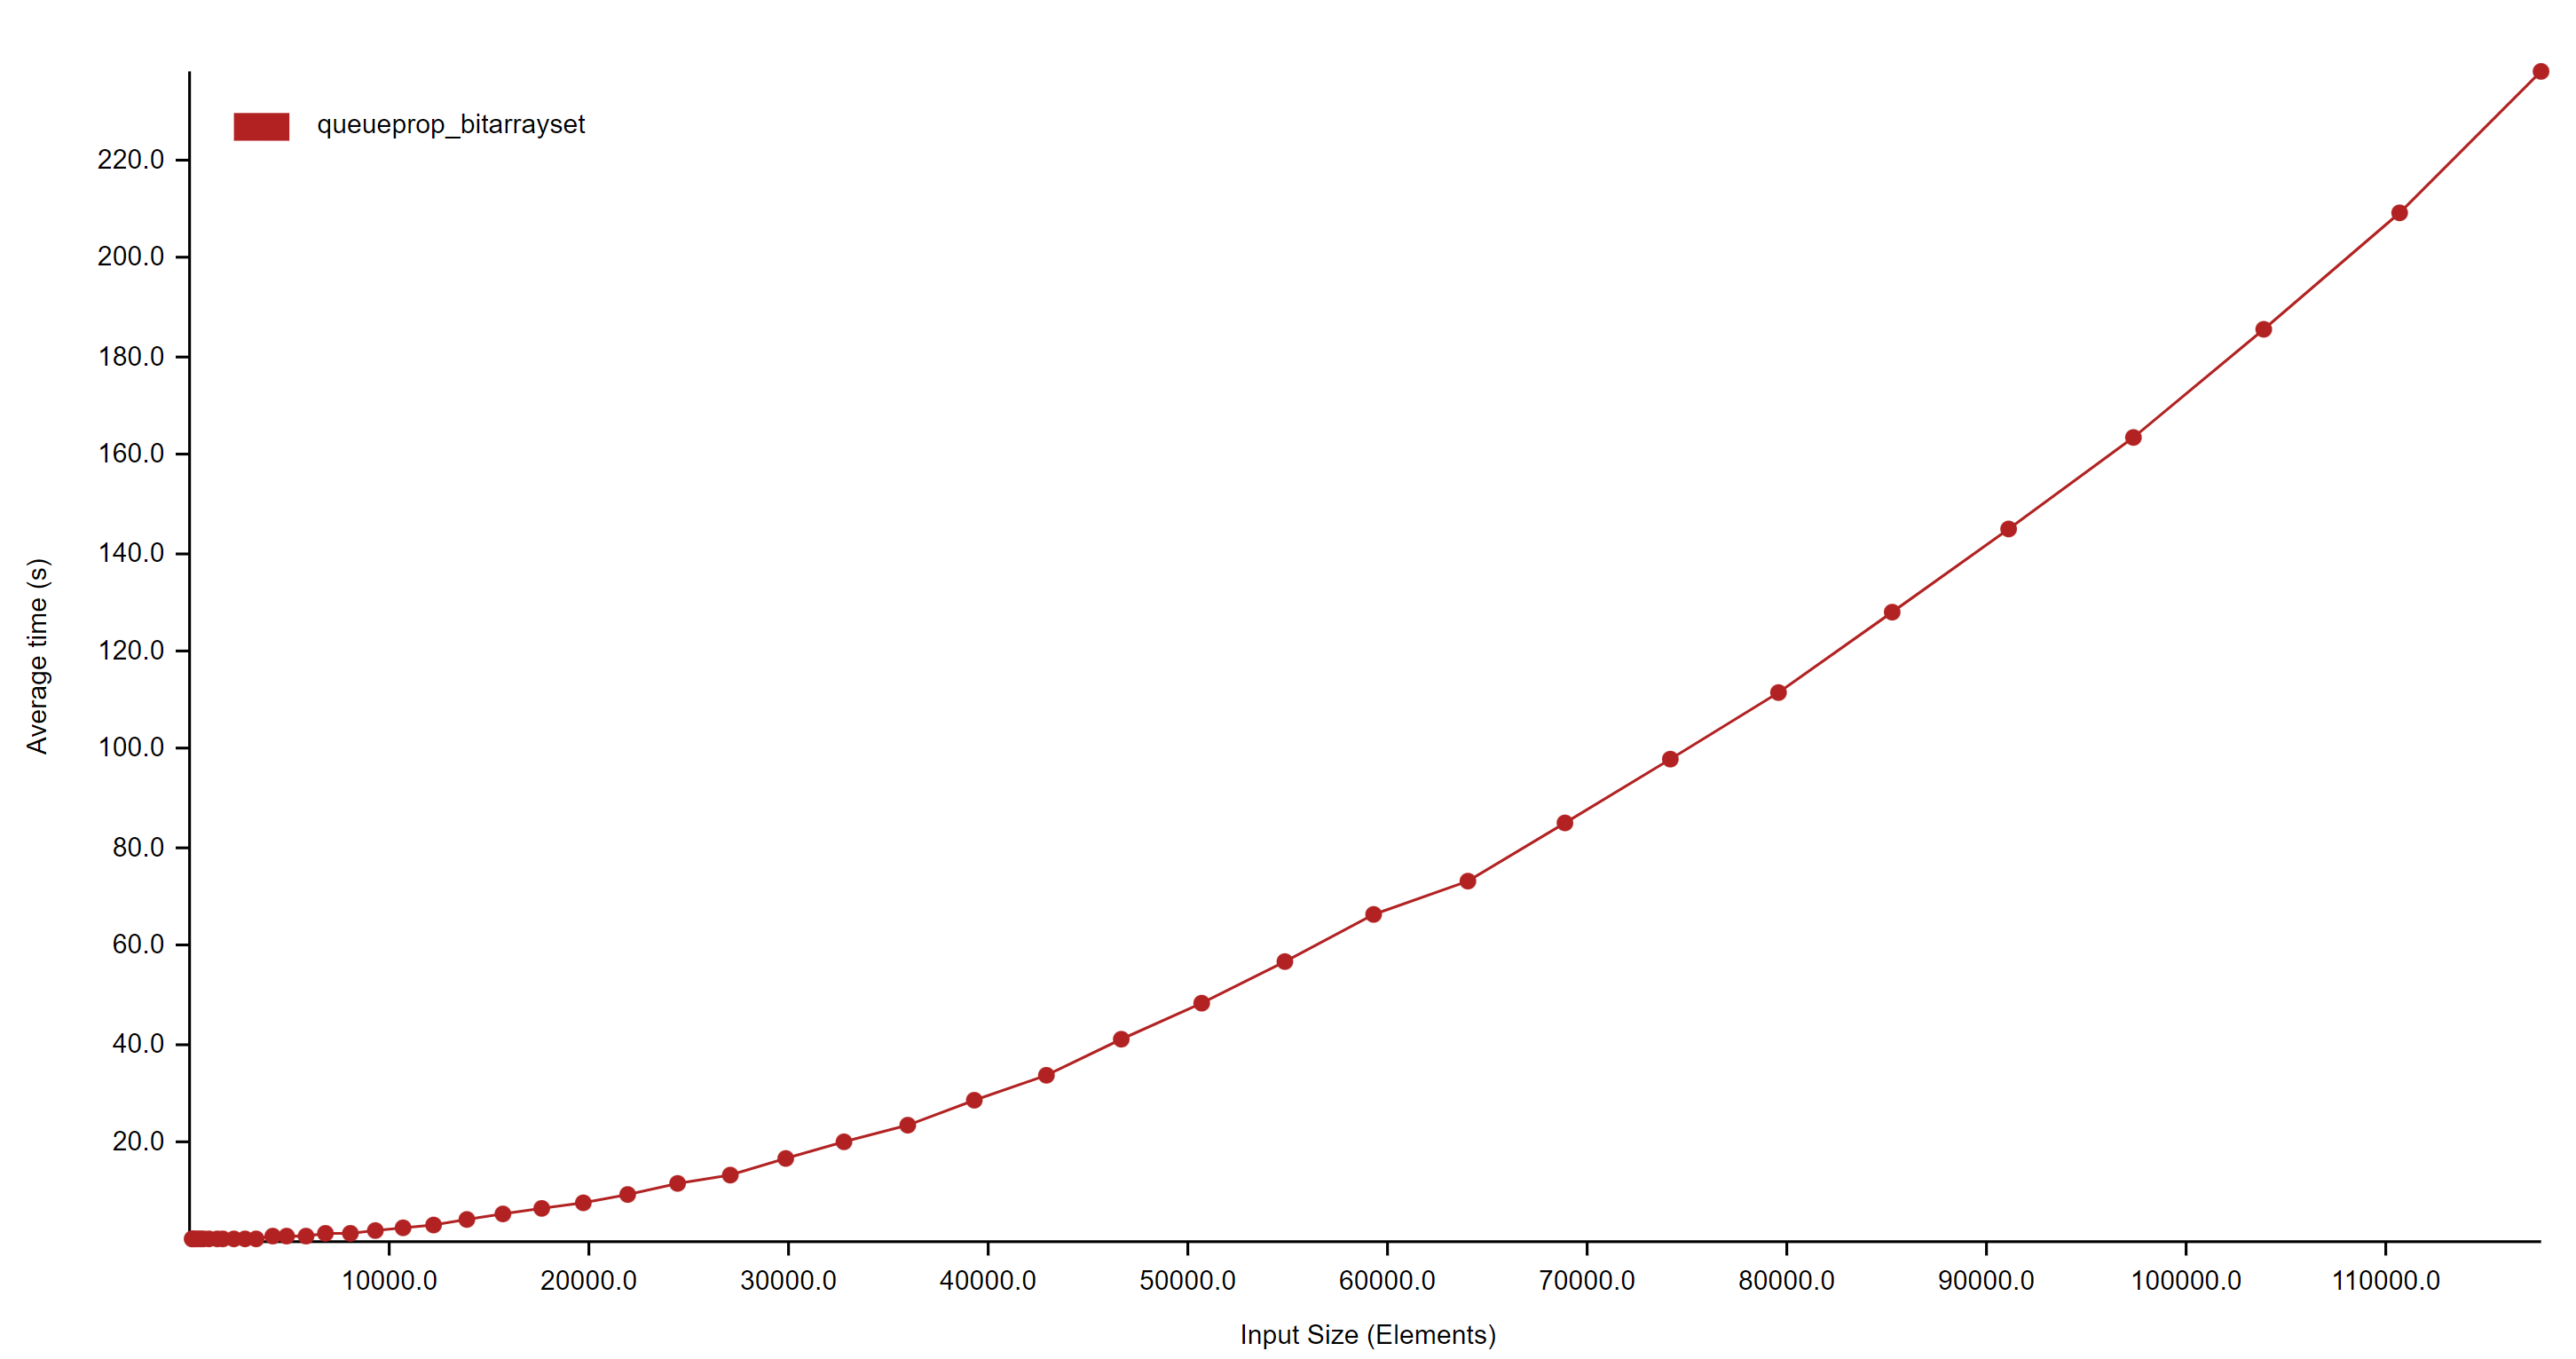
\includegraphics[width=1\textwidth, angle=0]{images/queueprop_bitarrayset_performance.png}
\caption{performance of the variant using bitwise operations}
\label{fig:queue_bitarrayset_performance}
\end{figure}
\label{bitwise}
\subsection{Code Analysis}
This variant changes original representation of possible assignments to bits - ones represent allowed values and zeros represent banned values. This slightly reduces memory usage, but more importantly allows us to write code that is easily optimised by the compiler.

\break\break\break
Operations supported by this set like structure:
\begin{enumerate}
    \item intersection of n sets - and \(n - 1\)  times
    \item union of n sets - or \(n - 1\)  times
    \item \label{ptclar}len - popcnt(hardware); \textbf{vectorized bit count}; shift, add
    \item remove - shift, negation, and
    \item insert - shift, and
    \item contains - shift, and
\end{enumerate}
In the point \ref{ptclar}, there are 3 alternatives (compiler results). In case of our implementation, compiler chooses vectorized bit count.

Updating possible assignments takes:
\begin{enumerate}
    \item getting rules for each neighbor \(\mathcal{O}(6m)\)
    \item union of \(m\) sets for each neighbor \(\mathcal{O}(6m^2/64)\)
    \item intersection \(\mathcal{O}(6m/64)\)
\end{enumerate}
Total \(\mathcal{O}(\frac{390m + 6m^2}{64})\), which is almost 64 times faster than without bitwise operations.

Similarly, the observation phase can benefit from this improvement, but it has to be assumed that domain size is constant so compiler can prepare optimized algorithm for it. If POPCNT instruction is available and used then the ones of a single word can be count in a single processor instruction. This makes this step 64 times faster for 64 bit processors (assuming POPCNT is done in one cycle\footnote{Lists of instruction latencies, throughputs and micro-operation breakdowns for Intel, AMD,
and VIA CPUs \url{https://www.agner.org/optimize/instruction_tables.pdf}}).

\begin{figure}
\begin{minted}{rust}
fn legal_tiles(x: usize, y: usize, z: usize, map: &Vec3D<Bits256Set>,
               rules: &Vec<DirectionMapping<Bits256Set>>) -> Bits256Set
{
    let dirs = vec![
        Bits256Set::new_sum(map.get(x,y+1, z)
                               .items()
                               .iter()
                               .map(|&s| *rules[s as usize].down())
                               .collect::<Vec<Bits256Set>>()),
        //... analogic operation done for other directions
    ];
    Bits256Set::new_intersection(dirs)
}
\end{minted}
\caption{function used to update a variable possible assignments}
\label{fig:legal_tiles_bits}
\end{figure}



\subsection{Performance}
Change in performance is seen only in propagation phase and it is a constant factor, but it still allows this variant to be almost 10 times faster than previous implementation for \(n = 39304\)(the largest benchmarked problem for variant using queue, see previous variant performance \ref{table:queue}).


\begin{table}[]
\centering
\begin{tabular}{@{}l|r|r|r|r|@{}}
\cmidrule(l){2-5}
                                 & \multicolumn{1}{c|}{Lower bound} & \multicolumn{1}{c|}{Estimate} & \multicolumn{1}{c|}{Upper bound} & \multicolumn{1}{c|}{Units} \\ \midrule
\multicolumn{1}{|l|}{Throughput} & 1.37                             & 1.38                          & 1.39                             & Kelem/s                    \\ \midrule
\multicolumn{1}{|l|}{Mean}       & 28.30                            & 28.49                         & 28.69                            & s                          \\ \midrule
\multicolumn{1}{|l|}{Std. Dev.}  & 151.83                           & 334.79                        & 448.11                           & ms                         \\ \midrule
\multicolumn{1}{|l|}{Median}     & 28.32                            & 28.41                         & 28.72                            & s                          \\ \bottomrule
\end{tabular}
\caption{the WFC algorithm with bitwise operations measured with \(n = 39304\)}
\label{table:bitwise}
\end{table}



\section{Fibonacci Heap For Faster Finding Of Lowest Non-Zero Entropy}
\begin{figure}[H]
\centering
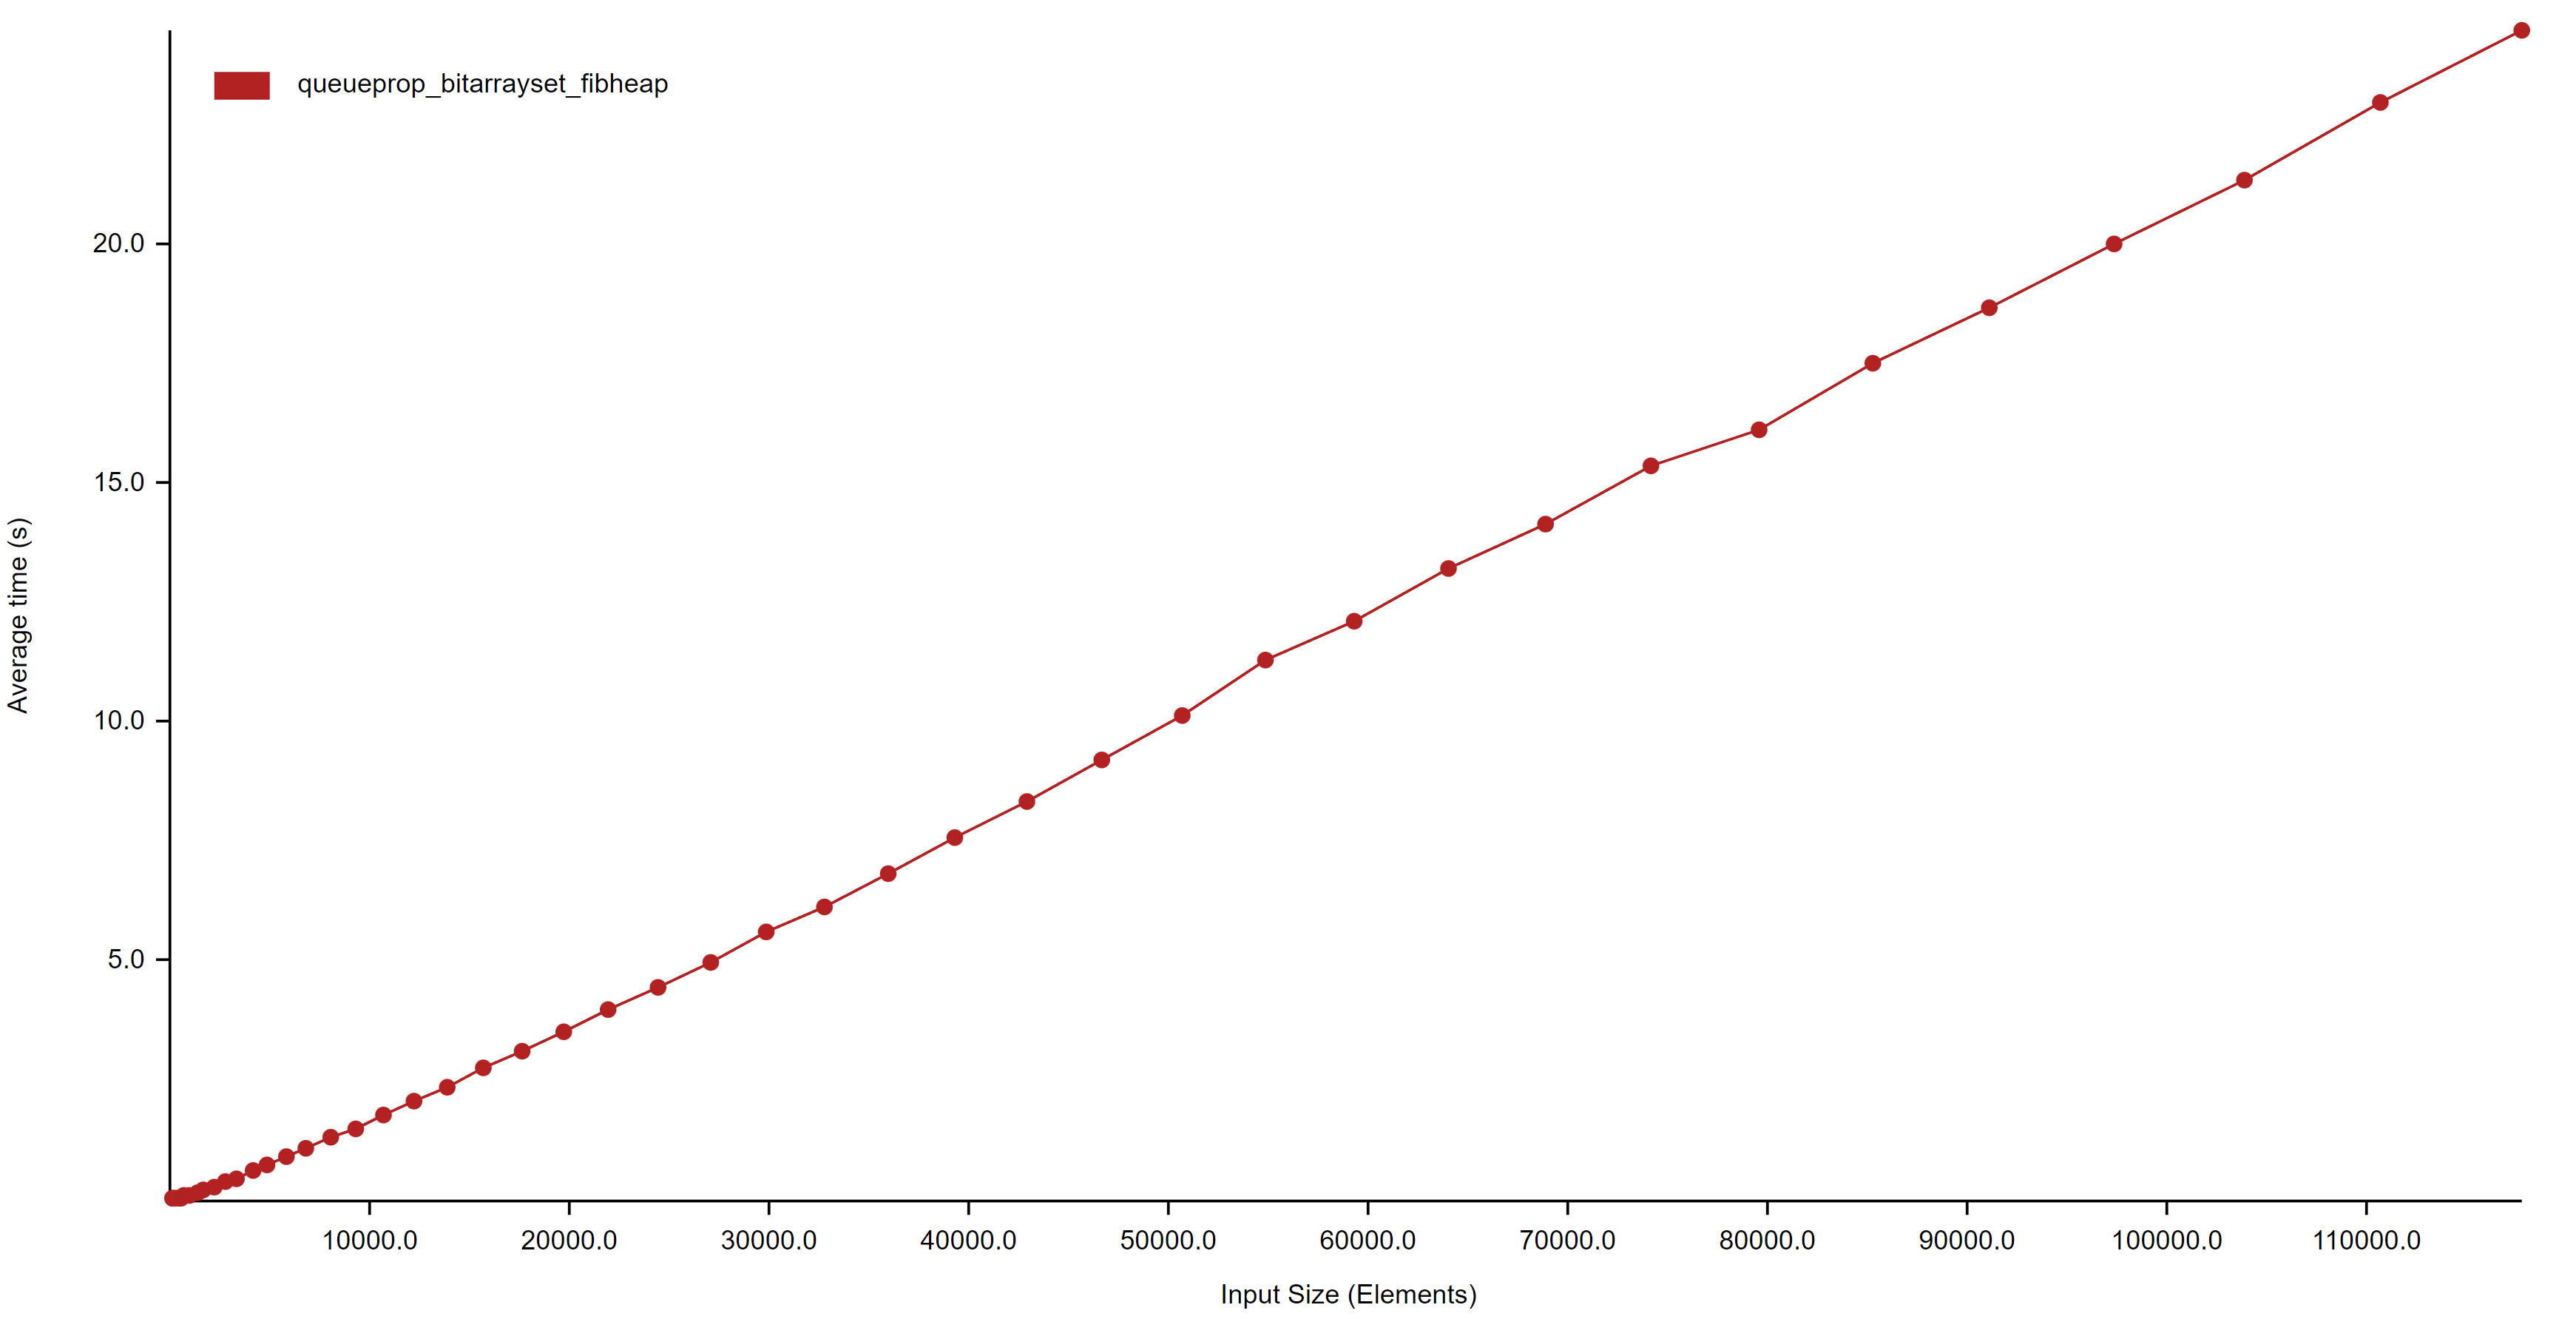
\includegraphics[width=1\textwidth, angle=0]{images/fibheap_performance.png}
\caption{performance of the variant using Fibonacci heap}
\label{fig:queue_bitarrayset_fibheap_performance}
\end{figure}
\label{fibheap}
\subsection{Code Analysis}
Fibonacci heap's pop min is \(\mathcal{O}(\log{n})\) amortized time, and decrease key is \(\mathcal{O}(1)\), this allows us to reduce time complexity of observation phase from \(\mathcal{O}(mn^2)\) to\break\(\mathcal{O}(n(m + \log{n}))\) and as a result the time complexity of this variant is \break\(\mathcal{O}(n(m + \log{n}) + n(72m^2 + 36m^3)) = \mathcal{O}(n(\log{n} + m + m^2 + m^3))\).

The algorithm uses the pop min operation to find a minimum non zero entropy and the decrease key operation while updating possible assignments.

\subsection{Performance}
\begin{figure}[H]
\centering
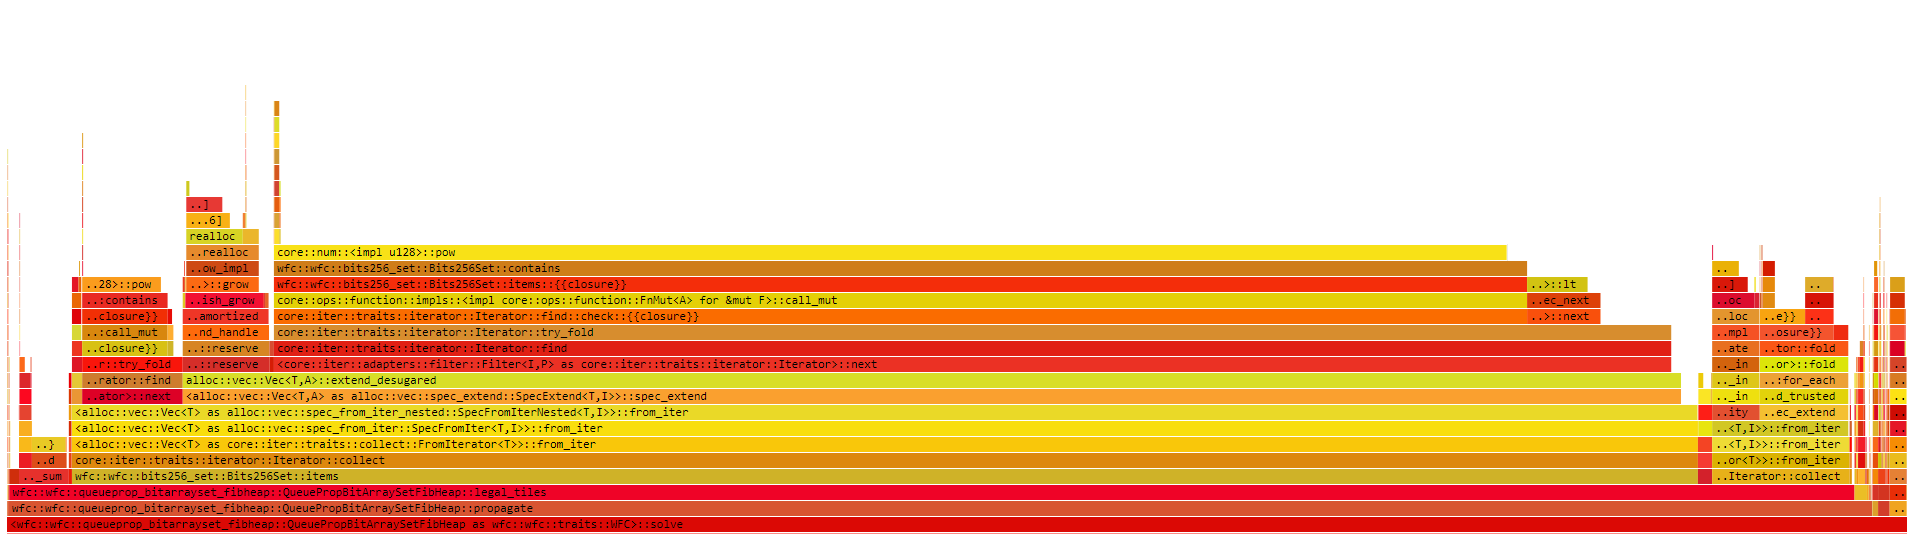
\includegraphics[width=1\textwidth, angle=0]{images/fibheap_flamegraph.png}
\caption{performance of the variant using Fibonacci heap}
\label{fig:fibheap_flamegraph}
\end{figure}
As shown in Figure \ref{fig:fibheap_flamegraph}, the observation phase (finding minimum) has negligible impact on performance in this version of the algorithm. It takes less than \(1\%\)  of the running time of the algorithm. Table \ref{tab:fibheap} presents results of this variant.

\begin{table}[]
\centering
\begin{tabular}{@{}l|r|r|r|r|@{}}
\cmidrule(l){2-5}
\multicolumn{1}{c|}{}            & \multicolumn{1}{c|}{Lower bound} & \multicolumn{1}{c|}{Estimate} & \multicolumn{1}{c|}{Upper bound} & \multicolumn{1}{c|}{Units} \\ \midrule
\multicolumn{1}{|l|}{Throughput} & 5.17                             & 5.19                          & 5.20                             & Kelem/s                    \\ \midrule
\multicolumn{1}{|l|}{Mean}       & 7.56                             & 7.58                          & 7.60                             & s                          \\ \midrule
\multicolumn{1}{|l|}{Std. Dev.}  & 18.34                            & 32.39                         & 40.84                            & ms                         \\ \midrule
\multicolumn{1}{|l|}{Median}     & 7.55                             & 7.58                          & 7.61                             & s                          \\ \bottomrule
\end{tabular}
\caption{the WFC algorithm with Fibonacci heap measured with \(n = 39304\)}
\label{tab:fibheap}
\end{table}

\chapter{Technical}
\label{chapter5}
\section{Installation Instruction}
\begin{enumerate}
    \item download code from repository \url{https://github.com/KrzysiekSlawik/wfc}
    \item compile code with: cargo build (--profile=release-with-debug if building for profiling)
    \item run tests: cargo test
    \item run benchmarks: cargo bench (it can take more than 12 hours)
\end{enumerate}

There are example targets in the repository that can be used to experiment with the algorithm. Each target uses different variant of the algorithm.

\section{Technologies Used}
\begin{enumerate}
    \item Rust programming language
    \item Criterion benchmarking library
    \item Cargo Flamegraph call stack visualization tool and Perf profiler
\end{enumerate}

\chapter{Future Work}
\label{chapter6}
\section{Custom Structure For Priority Queue}
\label{prioritybuckets}
Custom priority queue can be faster than well-known versions by exploiting the fact that in most use cases domain size is relatively small. One example is a bucket based structure. It can have one bucket for each priority (there are at most \(m\) priorities), and track non empty buckets using \(m\) bits. The same structure currently used for storing possible assignments can be utilized but should be extended with an index of the lowest bit. It can be implemented using the LZCNT instruction, which can be executed in a single cycle on some CPUs.


\section{Memory Locality}
\label{chunks}
To reduce cache misses we can align the array layout with the traversal order. One possible approach is to organize the problem into cache friendly chunks. The concept of chunking can be applied on multiple levels, by organizing problem into chunks of chunks. The size of chunks at each level should match the sizes of cache entries on different levels of cache.


\section{Backtracking}
Introduction of backtracking is crucial to make this algorithm reliable. For problems with strict rules, contradiction rate is high and thus preventing algorithm from finishing. Backtracking allows for gradual and steady progression towards the result.


\section{Additional Heuristics}
Currently these improvements have only been applied to the minimal working version of the WFC algorithm. To make it a robust tool for procedural generation, additional heuristics can be added. Implementing restrictions on density, count, and distance would provide better control over generated content.

\chapter{Summary}
\begin{figure}[H]
\centering
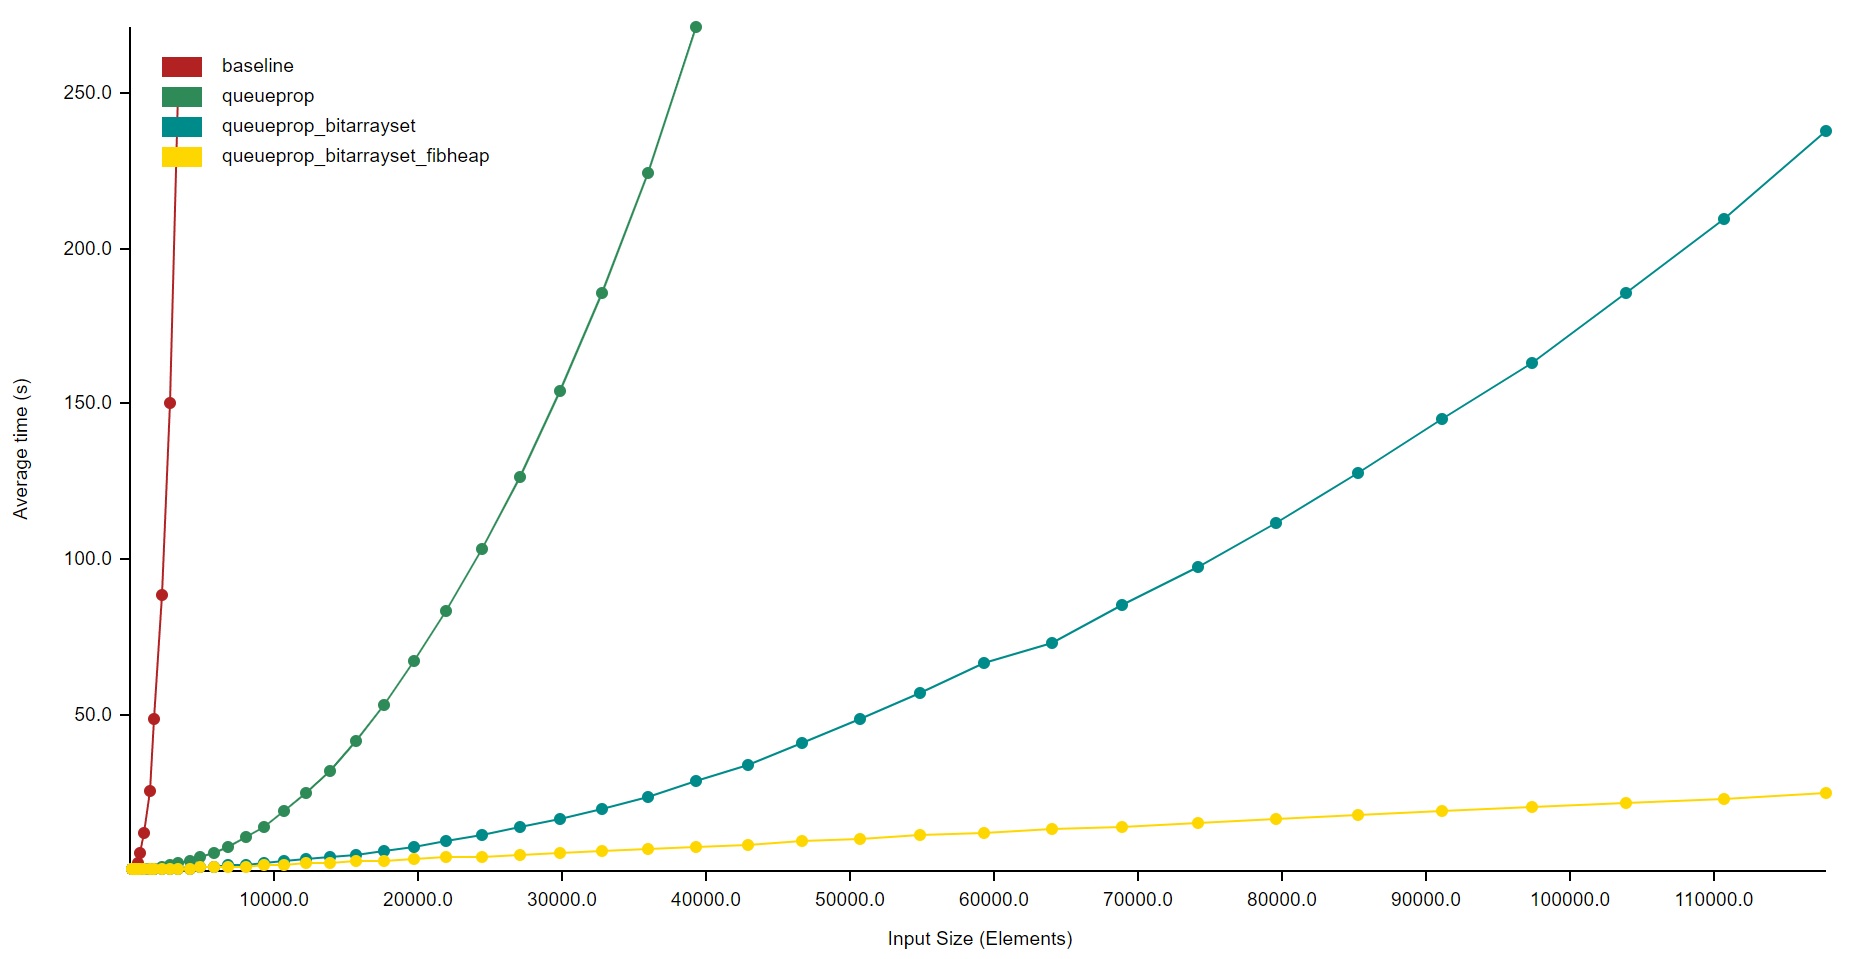
\includegraphics[width=1\textwidth, angle=0]{images/summary.png}
\caption{performance of the variant using Fibonacci heap}
\label{fig:summary}
\end{figure}
Our comparison shows the difference in  running time of four versions of the WFC algorithm, all of which are implemented in the Rust programming language. The first three are equivalents of existing solutions. For the purposes of this comparison, \(m\) is assumed to be a constant. Such an assumption is acceptable because for most practical applications this value does not exceed an insignificant constant.
\begin{enumerate}
    \item Baseline is an equivalent of Maxim Gumin's 2016 implementation. The time complexity is \(\mathcal{O}(n^2 + n^2)\).
    \item Queueprop is an equivalent of Maxim Gumin's implementation, but it uses a queue instead of a stack to track updates. The time complexity is \(\mathcal{O}(n + n^2)\).
    \item QueuepropBitarrayset is based on Oskar Stålberg's idea to use bitwise operators (implemented before reading the original idea). The time complexity is \(\mathcal{O}(n + n^2)\), but the constants are reduced substantially.
    \item \label{fibheap}QueuepropBitarraysetFibheap uses Fibonacci heap, which reduces the observation phase time complexity. The time complexity is \(\mathcal{O}(n + n\log{n})\).
\end{enumerate}
These improvements leads to faster content generation which could be important in creating game worlds, solving constraint satisfaction problems (CSPs), or synthesizing textures. Further improvements, should focus on the propagation phase, which currently takes the most time, by simplifying the representation of possible assignments and taking advantage of hardware optimizations like the POPCNT instruction.

Our method reduced run time by an order of magnitude. We improved the time complexity from \(\mathcal{O}(n^2)\) to \(\mathcal{O}(n + n\log{n})\), which enables the algorithm to operate on much larger scale.
\begin{figure}[H]
\centering
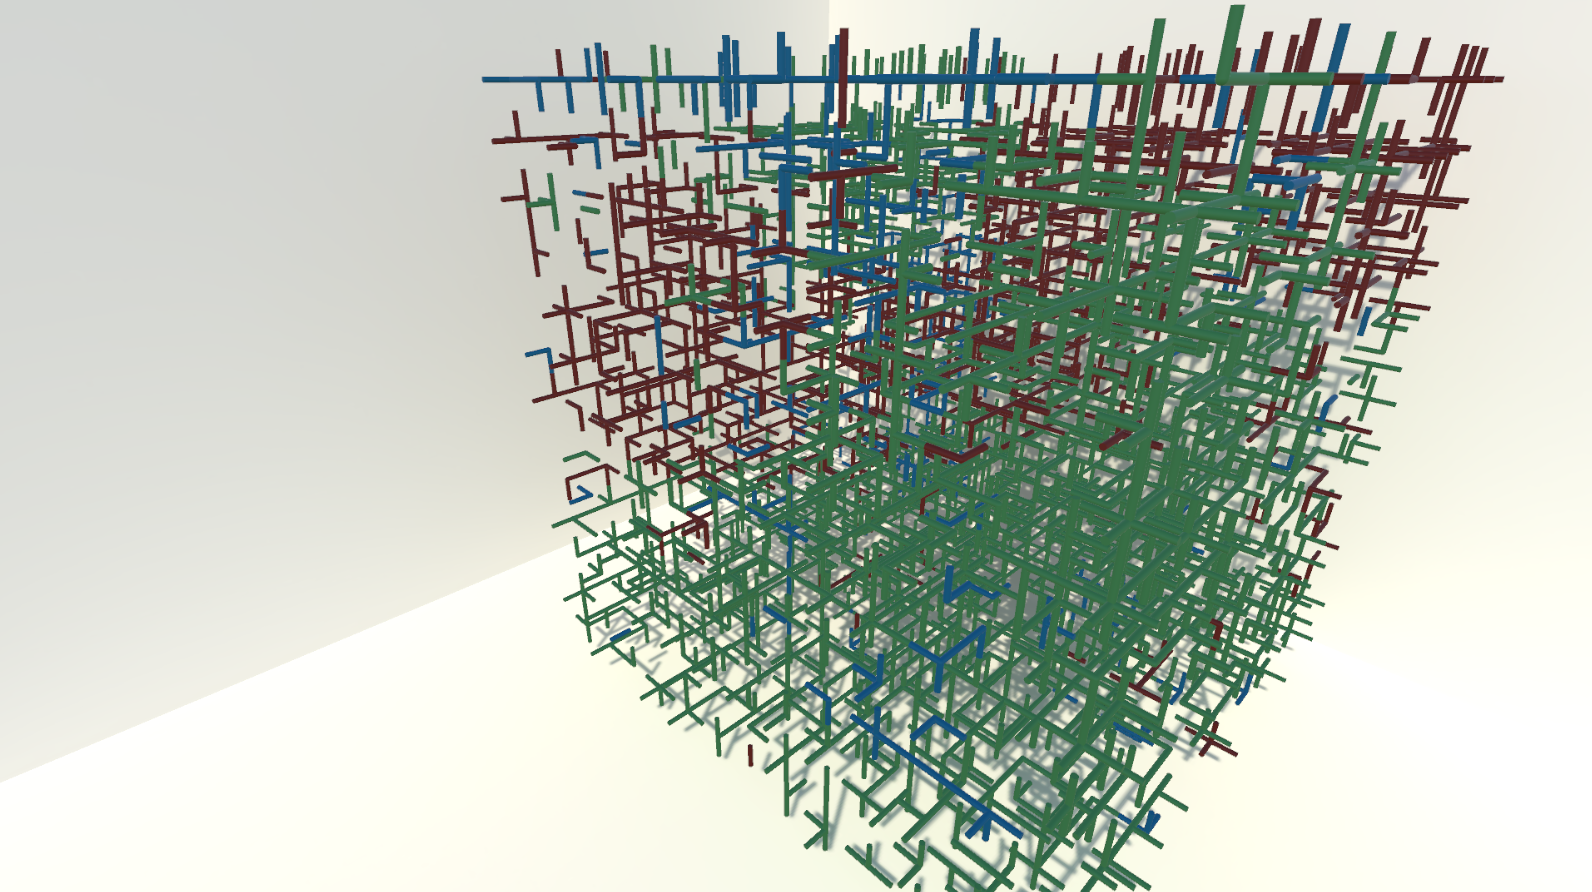
\includegraphics[width=1\textwidth, angle=0]{images/original_output.png}
\caption{The output of our version of WFC for the relaxed data set that was used for benchmarks}
\end{figure}

%%%%% BIBLIOGRAFIA
\printbibliography[sorting=none]

\end{document}
